\documentclass[12pt]{report} 
\usepackage[utf8]{inputenc}
\usepackage{geometry}
\geometry{letterpaper}
\usepackage{graphicx} 
\usepackage{parskip}
\usepackage{booktabs}
\usepackage{array} 
\usepackage{paralist} 
\usepackage{verbatim}
\usepackage{subfig}
\usepackage{fancyhdr}
\usepackage{sectsty}
\usepackage{bbm}
\usepackage[shortlabels]{enumitem}

\pagestyle{fancy}
\renewcommand{\headrulewidth}{0pt} 
\lhead{}\chead{}\rhead{}
\lfoot{}\cfoot{\thepage}\rfoot{}


%%% ToC (table of contents) APPEARANCE
\usepackage[nottoc,notlof,notlot]{tocbibind} 
\usepackage[titles,subfigure]{tocloft}
\renewcommand{\cftsecfont}{\rmfamily\mdseries\upshape}
\renewcommand{\cftsecpagefont}{\rmfamily\mdseries\upshape} %

\usepackage{amsmath}
\usepackage{amssymb}
\usepackage{mathtools}
\usepackage{empheq}
\usepackage{xcolor}

\usepackage{tikz}
\usetikzlibrary{positioning}
\usetikzlibrary{calc}

\usepackage{pgfplots}
\usepackage{tikz-cd}
\usepackage{tikz-qtree}
\pgfplotsset{compat=1.18}

\newcommand{\ans}[1]{\boxed{\text{#1}}}
\newcommand{\vecs}[1]{\langle #1\rangle}
\renewcommand{\hat}[1]{\widehat{#1}}

\newcommand{\F}{\mathcal{F}}
\renewcommand{\P}{\mathbb{P}}
\newcommand{\R}{\mathbb{R}}
\newcommand{\E}{\mathbb{E}}
\newcommand{\Z}{\mathbb{Z}}
\newcommand{\N}{\mathbb{N}}
\newcommand{\Q}{\mathbb{Q}}
\renewcommand{\L}{\mathbb{L}}
\renewcommand{\S}{\mathcal{S}}
\newcommand{\ind}{\mathbbm{1}}

\newcommand{\qed}{\quad \blacksquare}
\newcommand{\brak}[1]{\left\langle #1 \right\rangle}
\newcommand{\bra}[1]{\left\langle #1 \right\vert}
\newcommand{\ket}[1]{\left\vert #1 \right\rangle}
\newcommand{\abs}[1]{\left\vert #1 \right\vert}
\newcommand{\mfX}{\mathfrak{X}}
\newcommand{\ep}{\varepsilon}

\newcommand{\Cov}{\text{Cov}}
\newcommand{\Var}{\text{Var}}

\newcommand{\sub}{\subseteq}

\newcommand*{\tbf}[1]{\ifmmode\mathbf{#1}\else\textbf{#1}\fi}


\usepackage{tcolorbox}
\tcbuselibrary{breakable, skins}
\tcbset{enhanced}
\newenvironment*{tbox}[2][gray]{
    \begin{tcolorbox}[
        parbox=false,
        colback=#1!5!white,
        colframe=#1!75!black,
        breakable,
        title={#2}
    ]}
    {\end{tcolorbox}}

\newenvironment*{exercise}[1][red]{
    \begin{tcolorbox}[
        parbox=false,
        colback=#1!5!white,
        colframe=#1!75!black,
        breakable
    ]}
    {\end{tcolorbox}}

\title{APMA 1930X: Probability, Optimization, and Stochastic Calculus}
\author{Milan Capoor}
\date{Fall 2024}

\begin{document}
\maketitle
\chapter{Introduction and Examples}
\section*{Sept 04}
\subsection*{Kelly Betting}
    Imagine a game where 
    \[\begin{tikzcd}
        & 0.90 = 1.9\\ 
        1 \arrow[ur, "50\%"] \arrow[dr, "50\%"]&\\
        & -0.5 = 0.5
    \end{tikzcd}\]  

    So our expected payoff is 
    \[\E(\text{payoff}) = 0.5\cdot 0.9 + 0.5 \times (-0.5) = 0.2\]
    so the game is favorable to you. 

    Now consider the game 
    \[\begin{tikzcd}
        & 0.90x = 1.9x\\ 
        x \arrow["50\%"]{ur} \arrow["50\%"]{dr} &\\
        & -0.5x = 0.5x
    \end{tikzcd}\] 

    The expected payoff is
    \[\E[\text{payoff}] = 0.2x\]
    which is decidedly unfavorable. 

    Now betting all-in is not a good idea. Suppose your current wealth is $S_0$ and wealth after one bet is $S_1$ Consider the log of the second scenario:
    \[\begin{tikzcd}
        & \log(1.9 S_0) = \log(1.9) + \log(S_0)\\ 
        \log S_1 \arrow["50\%"]{ur} \arrow["50\%"]{dr}  &\\
        &  \log(0.5 S_0) = \log(0.5) + \log(S_0)
    \end{tikzcd}\]
    so 
    \[\begin{tikzcd}
        & \log(1.9)\\ 
        \log \frac{S_1}{S_0} \arrow["50\%"]{ur} \arrow["50\%"]{dr}  &\\
        &  \log(0.5 S_0) = \log(0.5)
    \end{tikzcd}\]

    Which tells us that after $n$ bets  
    \[\begin{tikzcd}
        & \log(1.9)\\ 
        \log \frac{S_n}{S_{n-1}} \arrow["50\%"]{ur} \arrow["50\%"]{dr}  &\\
        & \log(0.5)
    \end{tikzcd}\]

    Suppose that each bet is iid with $x_i = \log \frac{s_i}{s_{i-1}}$with $p(x_i = \log 0.5) = 0.5$and $p(x_i = \log 1.9) = 0.5$ Then 
    \[\log \frac{S_n}{S_{n-1}} + \log \frac{S_n-1}{S_{n-2}} + \cdots + \log \frac{S_1}{S_{0}} = X_n + X_{n-1} + \cdots + X_1\]
    hence 
    \[\log S_n = \log S_0 + (X_1 + \cdots + X_n)\] 
    By LLN 
    \begin{align*}
        \lim_{n \to \infty} \frac{1}{n} \sum_i x_i &= \E[X_1]\\ 
        &= 0.5 \log 1.9 + 0.5 \log 0.5\\
        &= 0.5 \log(0.95) < 0 
    \end{align*}
    so $S_n \to 0$ Clearly, all-in betting is not a good idea. 

    What if we bet a very small fraction of our wealth? By LLN, we will \emph{eventually} realize our edge but we will have to wait a long time. Can we do better?

    Now bet $wx$where $0 \leq w \leq 1$ Then 
    \[\begin{tikzcd}
        & x + 0.90wx\\ 
        x \arrow["50\%"]{ur} \arrow["50\%"]{dr} &\\
        & x - 0.5wx
    \end{tikzcd} \implies \begin{tikzcd}
        & \log(1 + 0.9w)\\
        \log \frac{S_n}{S_{n-1}} \arrow["50\%"]{ur} \arrow["50\%"]{dr} &\\
        & \log(1 - 0.5w)
    \end{tikzcd}\]
    so 
    \[\E[\log \frac{S_n}{S_{n-1}}] = 0.5 \log(1 + 0.9w) + 0.5(\log 1 - 0.5w)\] 
    which we want to maximize for $w \in [0, 1]$

    Taking the derivative, we get 
    \[\frac{0.9}{1  +0.9w} - \frac{0.5}{1 - 0.5w} = 0 \implies 0.9 - 0.45w = 0.5 + 0.45w\]
    so the best betting fraction is $w^* = \frac{4}{9}$and 
    \[\E(\log \frac{S_n}{S_{n-1}}) = 0.5\log \frac{9.8}{9} \approx 0.05\]

    We can graph our expected value function 

    \begin{center}
        \begin{tikzpicture}
            \begin{axis}[
                axis lines = middle,
                xlabel = $w$,
                domain=0:1,
                samples=100,
                ymin=-0.25, ymax=0.25,
            ]
            \addplot[
                blue,
                thick
            ]
                {0.5*ln(1 + 0.9*x) + 0.5*ln(1 - 0.5*x)};
            \addplot[red, thick, dotted, label=$w^*$]
                coordinates {(4/9, 0) (4/9, 0.05)};
            \node at (axis cs:4/9, 0.06) [anchor=west, red] {$w^*$};
            \end{axis}
        \end{tikzpicture}
    \end{center}

\subsection*{Probability Review}
    \textbf{Example:} Toss a fair coin $p(H) = p(T) = 0.5$n times. 

    What is the probability of getting an even number of heads? 

    One method is to argue by partitioning the sample space. 

    Alternatively, we can argue from the first toss: Let $x_n = p(\text{even \# of H after n tosses})$ Then after the first toss, 
    \begin{itemize}
        \item if we got heads: we need an odd number of heads in the next $n-1$tosses which happens with probability $1 - x_{n-1}$
        \item if we got tails: we need an even number of heads in the next $n-1$tosses which happens with probability $x_{n-1}$
    \end{itemize}

    Therefore, by the Law of Total Probability, 
    \[x_n = 0.5(1 + x_{n-1}) + 0.5(x_{n-1}) = 0.5\]
    
    We call this method \textbf{First step analysis}

\section{Sept 06}
    Last time we ended with an example of a fair coin tossed $n$times. How can we compute 
    \[x_n = P(\text{even \# H with n tosses})\]

    \textbf{Method 1:} Make a partitioning argument, taking advantage of the equal probabilities of heads and tails.

    \textbf{Method 2:} First step analysis.
    
    We argue that on the first toss, if we get heads, then the final probability we have an even number of heads is the same as the probability we have an odd number of heads after $n-1$tosses. If we get tails, then the probability we have an even number of heads is the same as the probability we have an even number of heads after $n-1$tosses.

    Using the law of total probability, we get
    \[x_n = \frac{1}{2}(1 - x_{n-1}) + \frac{1}{2}x_{n-1} = \frac{1}{2}\]

    \textbf{The Law of Total Probability:} 
    Consider the example 
    \[\begin{tikzcd}
        & E \arrow[r] &  P(B \; | \; E)\\
        \cdot \arrow[ur, "P(E)"] \arrow[dr, "P(E^c)"] \\
        & E^c \arrow[r] & P(B \; | \; E^c)
    \end{tikzcd}\]

    Then 
    \begin{tbox}{\textbf{Law of total Probability:}
        \[P(B) = P(E) P(B \; | \; E) + P(E^c)P(B \; | \; E^c)\]}
        \emph{Proof:} 
        \begin{align*}
            RHS &= P(E)P(B \; | \; E) + P(E^c)P(B \; | \; E^c)\\
            &= P(E)\frac{P(B \cap E)}{P(E)} + P(E^c)\frac{P(B \cap E^c)}{P(E^c)}\\
            &= P(B \cap E) + P(B \cap E^c)\\
            &= P(B)\\ 
            &= LHS
        \end{align*}
    \end{tbox}

    Consider a scenario with a biased coin with $p(H) = p$ and $p(T) = q$ Now 
    \begin{align*}
        x_n &= p(1 - x_{n-1}) + qx_{n-1}\\ 
        &= p + (q - p)x_{n-1}
    \end{align*}

    We want a special solution to this equation which is a constant in $n$, i.e. $x_n = c$ 

    We know $x_1 = P(T) = q$ 

    Start with the guess $c = \frac{1}{2}$ Then 
    \begin{align*}
        x_n &= p + (1 - 2p)x_{n-1}\\
        x_n - \frac{1}{2} &= p + (1 - 2p)x_{n-1} - \frac{1}{2}\\ 
        &= (1 - 2p)(x_{n-1} - \frac{1}{2})\\ 
        &= (1 - 2p)(1 - 2p)(x_{n-2} - \frac{1}{2})\\ 
        &= \cdots\\
        &= (1 - 2p)^{n-1}(x_1 - \frac{1}{2})\\
        &= (1 - 2p)^{n-1}(p - \frac{1}{2})
    \end{align*}
    so 
    \[\boxed{x_n = \frac{1}{2} + (1 - 2p)^{n-1}(q - \frac{1}{2}) = \frac{1}{2} + \frac{1}{2}(1 - 2p)^n}\]

    Thus, we can say the general method is 1) use first-step analysis to get a recursive formula and 2) guess a solution and prove it by induction.

    \textbf{Example (Putnam 2001):} We have $n$coins $C_1, C_2, \ldots, C_n$with $P(C_k = H) = \frac{1}{2k + 1}$ What is the probability that the number of heads is odd after tossing all $n$coins?

    Let's try the same approach as last time.

    Let $x_n = P(\text{odd \# of heads after n coins})$ Then the first toss gives us 
    \[x_1 = P(C_1 = H) = \frac{1}{3}\]
    \[\begin{tikzcd}
        & H\\
        C_{1} \arrow[ur, "\frac{1}{3}"] \arrow[dr, "\frac{2}{3}"] &\\
        & T 
    \end{tikzcd}\]
    But in fact this tells us nothing because the probability of getting an even number of heads in the next $n-1$ tosses is not $1 - x_{n-1}$ but some function of $\frac{1}{2k+1}$ 

    We actually need to start from the last toss:
    \[\begin{tikzcd}
        & H \arrow[r, dashed, no head] & 1 - x_{n-1} \quad \text{(even \# H in first (n-1) tosses)}\\ 
        x_{n} \arrow[ur, "{\frac{1}{2n+1}}"] \arrow[dr, "{\frac{2n}{2n+1}}"] &\\
        & T \arrow[r, dashed, no head] & x_{n-1} \quad \text{(odd \# H in first (n-1) tosses)}
    \end{tikzcd}\]

    So 
    \begin{align*}
        x_n &= \frac{1}{2n+1}(1 - x_{n-1}) + \frac{2n}{2n+1}x_{n-1}\\
        &= \frac{1}{2n+1} + \frac{2n - 1}{2n+1}x_{n-1}
    \end{align*}

    Again guessing $x_n = \frac{1}{2}$, 
    \begin{align*}
        x_n - \frac{1}{2} &= \frac{2n - 1}{2n + 1}(x_{n-1} - \frac{1}{2})\\ 
        &= \frac{2n - 1}{2n + 1}\frac{2n - 3}{2n - 1}(x_{n-2} - \frac{1}{2})\\
        &= \frac{2n - 1}{2n + 1}\frac{2n - 3}{2n - 1}\cdots \frac{3}{5}(x_{1} - \frac{1}{2})
        &= \cdots\\
        &= \frac{3}{2n+1}(\frac{1}{3}- \frac{1}{2})\\ 
        &= -\frac{1}{2(2n+1)}\\
        x_n &= \frac{1}{2} - \frac{1}{2(2n+1)} = \boxed{\frac{n}{2n + 1}}
    \end{align*}

    \textbf{Example (Law of Total Probability for Continuous RV)}: When we have finitely many possible outcomes, we can simply sum them by the LTP. What if we have infinitely many? 
    
    Consider a coin where $P(H) \sim \text{Unif}[0, 1]$ If we toss the coin $n$ times and define $X = $ \# of H, what is $P(X = k), k = 0, 1, \dots, n$?

    (Easier variation) Define $\theta = P(H) \sim \text{Unif}[0, 1]$ Suppose we are given $\theta = p$ Now 
    \[P(X = k \; | \; \theta = p) = \binom{n}{k} p^k (1 -p)^{n-k}\]

    For the continuous case, we have 
    \[P(X = k) = \int_0^1 P(X = k \; | \; \theta = p) \cdot (\text{density of } \theta \text{ at } p)\; dp\]

    But the density of $\theta$ at $p$ is simply 1 (uniform!). So
    \[P(X = k) = \int_0^1 \binom{n}{k} p^k (1 - p)^{n-k} \; dp\]
    
    Let's do some examples:
    \[P(X = 0) = \int_0^1 (1 - p)^n \; dp = \frac{1}{n + 1}\]
    (hint: change of variables $u = 1 - p$)

    \begin{align*}
        P(X = 1) &= \int_0^1 n p(1-p)^{n-1} \; dp\\ 
        &\overset{x = 1 - p}{=} \int_1^0 n(1 - x)x^{n1}\; (-dx)\\ 
        &= \int_0^1 nx^{n-1} - nx^n\; dx\\ 
        &= 1  - n \frac{1}{n + 1} = \frac{1}{n + 1}
    \end{align*}

    \begin{align*}
        P(X = n) = \int_0^1 p^n \; dp = \frac{1}{n + 1}
    \end{align*}

    So we conclude $P(X = k) = \frac{1}{n + 1}$

\section{Sept 09}
    Last time we introduced the \emph{continuous version of the Law of Total Probability}:
    \[P(A) = \int P(A \; | \; X = x) f_X(x)\; dx\]

    \textbf{Example:} Suppose you have a fair die ($X \in 1...6$). 
    \begin{enumerate}
        \item What is the average number of tosses until 6 appears?
        \item What is the average cumulative sum ($\sum x_i$) until 6 appears?
    \end{enumerate}

    Every time we toss the die, we know $P(6) = \frac{1}{6}$ and $P(\lnot 6) = \frac{5}{6}$. If $X$ is the number of tosses until 6, we know 
    \[X \sim \text{geometric}(p) \implies \E[X] = \frac{1}{p}\]

    Which we can see from 
    \begin{align*}
        \E[X] &= \sum_{i=1}^n P(X = n) \cdot n\\ 
        &= \sum_{i=1}^n (1- p)^{n-1} p \cdot n\\ 
        &\vdots\\ 
        &= \frac{1}{p}
    \end{align*}

    This method presents some difficulties in general: How do we explicitly know $P(X = n)$. Further, this method tells us nothing about question 2. 

    Let's try again with FSA: Let $X$ be the average number of tosses until 6. 

    Look at the first toss:

    \begin{center}
        \begin{tabular}{|p{1in}p{1in}|}
            \hline\\
            \multicolumn{2}{c}{1st Toss}\\ 
            Outcome on first toss & Average number of tosses to reach 6\\ 
            \hline
            1 & $x$\\ 
            2 & $x$\\ 
            3 & $x$\\ 
            4 & $x$\\ 
            5 & $x$\\ 
            6 & $0$\\ 
            \hline
        \end{tabular}
    \end{center}
   

    So 
    \[X = 1 + \frac{5}{6}x + \frac{1}{6}\cdot 0 = 1 + \frac{5}{6}X \implies \boxed{X = 6}\] 
    (the $1$ is the first toss we already used) 

    Now let $Y$ be the average cumulative sum until 6. We can draw exactly the same table because for each case the average depends on all the rest: 
    
    \begin{center}
        \begin{tabular}{|p{1in}p{1in}|}
            \hline\\
            \multicolumn{2}{c}{1st Toss}\\ 
            Outcome on first toss & Average number of tosses to reach 6\\ 
            \hline
            1 & Y\\ 
            2 & Y \\ 
            3 & Y\\ 
            4 & Y\\ 
            5 & Y\\ 
            6 & 0\\ 
            \hline
        \end{tabular}
    \end{center}
    
    so 
    \begin{align*}
        Y &= \frac{1}{6}(1 + y) + \frac{1}{6}(2 + y) + \cdots + \frac{1}{6}(5 + y) + \frac{1}{6}(6 + 0)\\ 
        &= \frac{5}{6}y + \frac{7}{2}\\ 
        &= 21
    \end{align*}

    \textbf{Example:} Toss a coin $n$ times and let $P(H) = p$. What is the probability that the pattern $HH$ does not appear? 

    Let $x_n$ be the probability that $HH$ does not appear after $n$ tosses. Then we know 
    \begin{align*}
        x_1 &= 0\\ 
        x_2 &= 1 - p^2
    \end{align*}
    but the rest become very complicated. 

    For simplicity, let $P(T) = q = 1 - p$.

    \begin{center}
        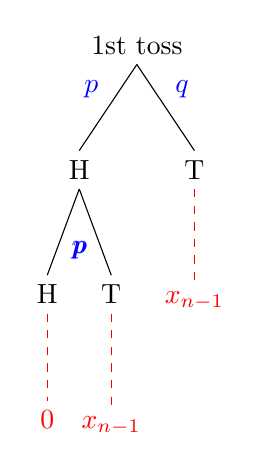
\begin{tikzpicture}[level distance=45]
            \Tree [.{1st toss} 
                    \edge node[auto=right, blue]{$p$}; [.H
                        \edge node[auto=left, blue]{$p$}; [.H \edge[dashed, red, auto=right]; \node[red]{0};] 
                        \edge node[auto=right, blue]{$p$}; [.T \edge[dashed, red, auto=right]; \node[red]{$x_{n-1}$};]]
                    \edge node[auto=left, blue]{$q$}; [.T \edge[dashed, red, auto=right]; \node[red]{$x_{n-1}$};]
                ]
        \end{tikzpicture}
    \end{center}

    So 
    \[x_n = qx_{n-1} + pqx_{n-2}, \quad x_1 = 1, x_2 = 1 - p^2\]

    We can solve this using a method similar to 2nd order ODEs: 
    \[f'' + af' + bf =0 \implies r^2 + ar + b = 0 \implies f = C_1e^{r_1 t} + C_2e{r_2 t}\]

    In our case 
    \[x_n = qx_{n-1} + pqx_{n-1} \implies r^2 = qr + pq\]

    We can find roots $r_1, r_2$ and then solve for $C_1, C_2$ using the initial conditions, giving our solution:
    \[\begin{cases}
        x_n = Ar_1^n + Br_2^n\\ 
        x_1 = 1, \; x_2 = 1- p^2
    \end{cases}\]

    \textbf{Example:} We are playing a game of dice with the following rules:

    \begin{enumerate}
        \item If the toss is 1, 2, 3, you get the face value and continue 
        \item If the toss is 4, 5, you get the face value and the game ends
        \item If the toss is 6, the game ends 
    \end{enumerate}

    \emph{Example game:} $3 \to 2 \to 2 \to 4$ gives score $11$

    What is the average payoff $x$? 
    \begin{center}
        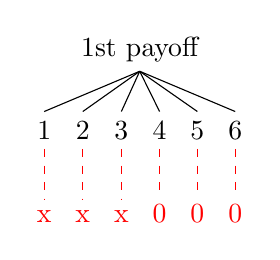
\begin{tikzpicture}
            \Tree [.{1st payoff}
                [.1 \edge[red, dashed]; \node[red]{x};] 
                [.2 \edge[red, dashed]; \node[red]{x};] 
                [.3 \edge[red, dashed]; \node[red]{x};] 
                [.4 \edge[red, dashed]; \node[red]{0};]
                [.5 \edge[red, dashed]; \node[red]{0};] 
                [.6 \edge[red, dashed]; \node[red]{0};]]
        \end{tikzpicture}
    \end{center}

    So 
    \[x = \frac{1}{6}(1 + x) + \frac{1}{6}(2 + x) + \frac{1}{6}(3 + x) + \frac{1}{6}(4 + 0) + \frac{1}{6}(5 + 0) + \frac{1}{6}(0) = 5\]

\section{Sept 11}
    \textbf{Harder Variation:} now the game rules are 
    \begin{enumerate}
        \item If the toss is 1, 2, 3, you get the face value and continue 
        \item If the toss is 4, 5, you get the face value and the game ends
        \item If the toss is 6, the game ends and you lose all your points
        \item You can stop the game whenever you want 
    \end{enumerate}

    Let $y$ be the average cumulative sum. Now 

    \begin{center}
        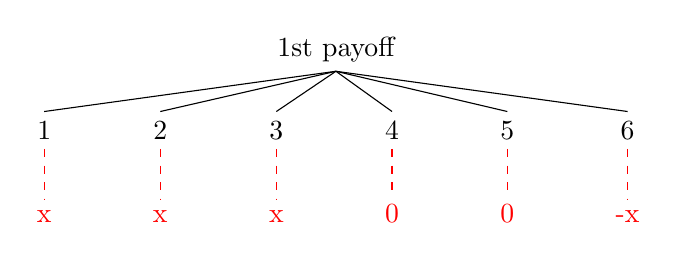
\begin{tikzpicture}[sibling distance=30pt]
            \Tree [.{1st payoff}
                [.1 \edge[red, dashed]; \node[red]{x};] 
                [.2 \edge[red, dashed]; \node[red]{x};] 
                [.3 \edge[red, dashed]; \node[red]{x};] 
                [.4 \edge[red, dashed]; \node[red]{0};]
                [.5 \edge[red, dashed]; \node[red]{0};] 
                [.6 \edge[red, dashed]; \node[red]{-x};]]
        \end{tikzpicture}
    \end{center}

    Recall that in the previous case where the game ended on 6 but you retained your score, 
    \[x = \frac{1}{6}(1 + x) + \frac{1}{6}(2 + x) + \frac{1}{6}(3 + x) + \frac{1}{6}(4 + 0) + \frac{1}{6}(5 + 0) + \frac{1}{6}(0) = 5\]

    However, in the new game this is not quite right: we are not guaranteed to keep our early points if we continue. What is the probability we keep our points? $2/3$ because out of the three ending conditions, we keep our points in two of them.

    So 
    \[y = \frac{1}{6}(\frac{2}{3} + y) + \frac{1}{6}(\frac{4}{3} + y) + \frac{1}{6}(2 + y) + \frac{1}{6}(4) + \frac{1}{6}(5) \implies \boxed{y = \frac{13}{3}}\]

    But this really only works because the stopping condition is simple. 

    \textbf{Example (Prison Dilemma):} 100 prisoners are given a chance to play a game for their freedom. There are 100 boxes that each contain a paper with a number from 1 to 100. Each prisoner has a number 1-100 and is allowed to open 50 boxes. If one of these 50 boxes contain his number, he wins. If all 100 prisoners win, they all go free. If anybody loses, they are all executed. 

    We know that if each prisoner opens boxes at random, the probability of winning is $\frac{1}{2^{100}}$. Can they do better?

    Here is one strategy, though we can't say if it is optimal: 
    \begin{enumerate}
        \item Each player opens the box corresponding to their number
        \item If they don't win, they open the box corresponding to the number on the paper in the box they just opened
        \item Repeat until they win or they have opened 50 boxes
    \end{enumerate}

    We are looking for cycles in the graph. If the cycle has length at most 50, everyone in the cycle wins. If the cycle is longer than 50, everyone loses.
    
    As cycles are disjoint, we can partition the space. Then everyone will win if all the cycles are of length at most 50 so 
    \begin{align*}
        \P(\text{win}) &= \P(\text{every cycle } \leq 50)\\
        &= 1 - \P(\text{at least one cycle} > 50)\\ 
        &= 1 - \P(\text{exactly one cycle} > 50)
    \end{align*}

    Let's look more generally: for $2n$ boxes what is the probability one cycle is of length at least $n$?
    \[\P(\text{one cycle } > n) = \sum_{k={n+1}}^{2n} \P(\text{one cycle} = k)\]

    We can view the contents of the boxes in order as a permutation of $2n$ elements. We know there are $(2n)!$ permutations. How many give a cycle of length $k$?

    Clearly, we want to choose $k$ elements to be in the cycle and then permute the rest. So
    \[\binom{2n}{k}(2n - k)!\]
    But how many ways are there to make a cycle with $\binom{2n}{k}$ elements? $(k-1)!$ 

    All together, 
    \begin{align*}
        \P(\text{one cycle} = k) &= \frac{1}{(2n)!} \binom{2n}{k}(2n - k)!(k-1)!\\ 
        &= \frac{1}{(2n)!}\frac{(2n)!}{(2n -k)!k!} (2n-k)!(k-1)!\\ 
        &= \frac{(k-1)!}{k!}
    \end{align*}

    So 
    \[\P(\text{win}) = 1 - \sum_{k=n+1}^{2n} \frac{1}{k}\]

    We can approximate 
    \[1 + \frac{1}{2} + \frac{1}{3} + \cdots + \frac{1}{n} = \log n + C\]
    for a constant $C$ so 
    \begin{align*}
        \P(\text{win}) &= 1 - \sum_{k=n+1}^{2n} \frac{1}{k}\\ 
        &= 1 - \left(\sum_{k=1}^{2n} \frac{1}{k} - \sum{k=1}^n \frac{1}{k}\right)\\ 
        &\approx 1 - (\log 2n + C - (\log n + C))\\ 
        &= 1 - \log 2 \approx 0.3
    \end{align*}

\section{Sept 13:}
\subsection*{Law of Total Expectation}
    \textbf{Example:} In America, 50.5\% of the population is female, 49.5\% is male. The average life expectancy is 79.1 for women and 73.2 for men. What is the average life expectancy of an American?

    \begin{align*}
        \frac{1}{N} \sum_{\text{Americans}} \text{life expectancy} &= \frac{1}{N} \sum_{\text{Women}} \text{life expectancy} + \frac{1}{N} \sum_{\text{Men}} \text{life expectancy}\\
        &= \frac{1}{N}(0.505N \cdot 79.1) + \frac{1}{N}(0.495N \cdot 73.2)\\
        &= 76.2
    \end{align*}
    or, in general, 
    \[P(A) = \sum_y P(A \; | \; Y = y)P(Y = y)\]

    This is incredibly intuitive but let's generalize. Say $Y$ is the average life expectancy of an American and $X$ is their sex. Let $X = 1$ if woman, $X =0$ if man. 
    Then the situation is expressed 
    \[\begin{cases}
        \P(X = 1) = 50.5\%, \quad \P(X = 0) = 49.5\%\\ 
        \E[Y \; | \; X = 1] = 79.1, \quad \E[Y \; | \; X = 0] = 73.2
    \end{cases}\]  


    Therefore, if we define a random variable $\E[Y \; | \; X]$ such that it takes value $\E[Y \; | \; X = 1]$ on event $X = 1$ and $\E[Y \; | \; X = 0]$ on event $X = 0$, then
    \[\E[Y] = \E[Y \; | \; X=1] \P(X = 1) + \E[Y \; | \; X = 0] \P(X = 0) = \E[\E[Y \; | \; X]]\]
    
    For $Y$ discrete, 
    \[\E[Y] = \E[\E[Y \; | \; X]] = \sum_y \E[X \; | \; Y = y] \P(Y = y)\]

    We call $E[Y \; | \; X]$ the \emph{conditional expectation} of $Y$ given $X$. 

    The Law of Total Expectation is a Generalization of the law of total probability. 

    Define for all $A \sub \Omega$, the \emph{indicator random variable} by
    \[\ind_{A}(\omega) = \begin{cases}
        1 & \omega \in A\\
        0 & \omega \notin A
    \end{cases}\]  

    Then, straightforwardly, $\P(A) = \E[\ind_A]$ and the Law of Total Probability is 
    \[\P(A) = \E \; | \; \P(A \; | \; X)\] 
    for any family of random variables $X$. 
    
    When $X$ is a single random variable: 
    \begin{align*}
        \P(A) &= \sum_i \P(A \; | \; X = x_i) \P(X = x_i)\\ 
        \P(A) &= \int_{\R} \P(A \; | \; X= x) f_X(x)\; dx
    \end{align*}
    depending on whether $X$ is discrete or continuous.

    \textbf{Example:} Sample $X_1, X_2, \dots, X_n \sim \text{Unit}[0, 1]$. Let $X_{(1)} = \min \{X_i$\}, $X_{(2)} = \min\{X_i \; | \; X_i \neq X_{(1)}\}$, etc.

    Then $X_{(1)} \leq X_{(2)} \leq \cdots \leq X_{(n)}$ is a rearrangement of $\{X_1, X_2, \dots, X_n\}$ is ascending order, what we call \emph{the order statistics} 

    These $n$ points now partition $[0, 1]$ into $(n+1)$ pieces. What is the average length of each piece? 

    It suffices to find the density of $X_{(1)}$ and compute $\E[X_{(1)}]$ and then compute the average length of each subinterval.

    First, we calculate the CDF:
    \[F_1(x) = \P(X_{(1)} \leq x) = 1 - \P(X_{(1)} > x) = 1 - (1 - x)^n\] 

    Then the density is
    \[f_1(x) = F_1'(x) = n(1-x)^{n-1} \cdot \ind_{[0, 1]}(x)\] 
    and 
    \begin{align*}
        E[X_{(1)}] &= \int_{\R} x f_1(x) \; dx\\ 
            &= \int_0^1 x n(1-x)^{n-1} \; dx\\
            &= \int_0^1 n(1 - t)t^{n-1}\; dt\\ 
            &= \int_0^1 n(t^{n-1} - t^n)\; dt\\ 
            &= 1 - \frac{n}{n+1}\\ 
            &= \frac{1}{n+1}
    \end{align*}

    The first piece on $[0, 1]$ is $[0, X_{(1)}]$ which has average length $\E[X_{(1)}] = \frac{1}{n + 1}$. 

    What about the second piece? 
    \begin{align*}
        \E[X_{(2)}] &= \E[\E[X_{(2)} \; | \; X_{(1)}]] \\ 
        &= \E[\frac{1}{n}(1 - X_{(1)})]\\ 
        &= \frac{1}{n} - \frac{1}{n}\E[X_{(1)}]\\
        &= \frac{1}{n}\left(1 - \frac{1}{n(n+1)}\right)\\
        &= \frac{1}{n+1}
    \end{align*}

    Repeating this procedure, we can see that each interval has average length $\frac{1}{n+1}$

\section{Sept 9}
\subsection*{Optimization}
        \textbf{Classic Optimization:} Given a sequence or function, find its max/min 

        \emph{Method:} Take the derivative and set it equal to zero.

        \textbf{Constrained Optimization:} e.g. maximize $f(x)$ given $g(x) = 0$

        \emph{Method:} Lagrange Multipliers 

        \textbf{Infinite Dimensional Problems:} e.g. $\max_f \, H(f)$ (where $H$ is a function of functions or a \emph{functional})

        \emph{Method:} Calculus of Variations
    
        \textbf{Example (Application of indicator RVs):} A company has $n$ employees. Anyone can take the day off if it is the birthday of some employee. Every work day is 8 hours. How many employees should the company hire so that the total working hour from employees is maximized? 
        
        Denote $a_n = \E[\text{total working hours with } n \text{ employees}]$. We then want to find $\max_n a_n$.

        Suppose $X$ is the total number of working days from $n$ employees. Then $a_n = \E[8Xn] = 8n\E[X]$

        But this distribution is very difficult to determine. Let's use indicator random variables. Let $X_{1}, X_2, \dots, X_{365}$ be RVs defined by 
        \[X_k = \begin{cases}
            1 & \text{if the k-th day is a working day}\\ 
            0 & \text{otherwise}
        \end{cases}\] 

        Then $X = X_1 + X_2 + \cdots + X_{365}$ is the total number of working days. So 
        \[\E[X] = \sum_{k=1}^{365} \E[x_k]\]

        But $x_k$ is a discrete RV so 
        \begin{align*}
            \E[x_k] &= 1 \cdot P(x_k = 1) + 0 \cdot P(x_k = 0)\\ 
            &= P(x_k = 1)\\ 
            &= \P(k \text{-th day is a working day })\\ 
            &= \P(k \text{-th day is no one's birthday})\\ 
            &= \prod_{i=1}^n \P(k \text{-th day is not the birthday of employee } i)\\
            &= \left(\frac{364}{365}\right)^n 
        \end{align*}

        Therefore, our problem reduces to maximizing 
        \[a_n = 8n \E[X] = 8n \cdot 365 \left(\frac{364}{365}\right)^n\]
        with respect to $n$.

        Consider $T_n = n \left(\frac{364}{365}\right)^n$. Then 
        \[\frac{T_{n+1}}{T_n} = \frac{(n + 1) \left(\frac{364}{365}\right)^n}{n\left(\frac{364}{365}\right)^n} = \frac{n + 1}{n} \cdot \frac{364}{365}\]
        
        Which is greater than 1 for $n < 365$, $< 1$ for $n > 365$, and equal to 1 for $n = 365$. 

        This tells us that $T_n$ is increasing for $n < 365$, decreasing for $n > 365$, and constant for $n = 364 \text{ or } 365$. Therefore, the optimal $n^* = 364$ or $365$.

        \textbf{Example (function maximization):} 
        \begin{enumerate}
            \item max/min $f(x)$ by solving $f'(x^*) = 0$ for $x^*$ 
            \item max/min $f(x, y)$ by solving $f_x = f_y = 0$ 
        \end{enumerate}

        \textbf{Example (Lagrange multipliers):} maximize $x + y$ given $x^2 + y^2 =1$ 

        Graphically: 
        \begin{center}
            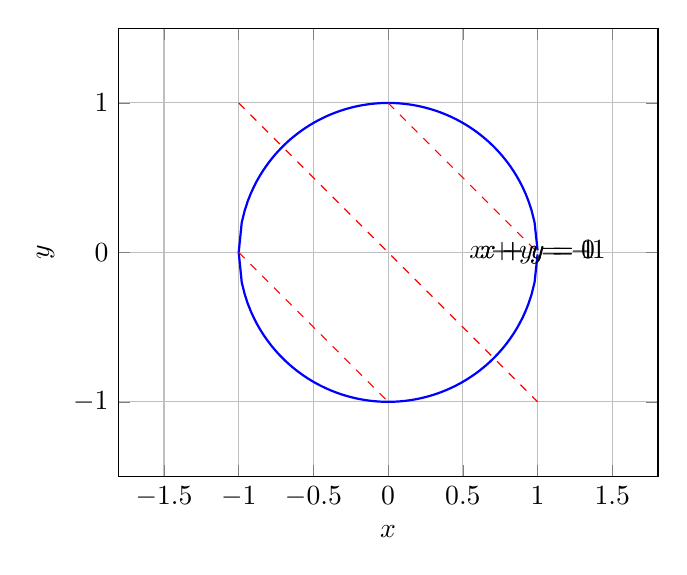
\begin{tikzpicture}
                \begin{axis}[
                    axis equal,
                    xlabel={$x$},
                    ylabel={$y$},
                    grid=major,
                    domain=-3:3,
                    xmin=-1.5, xmax=1.5,
                    ymin=-1.5, ymax=1.5,
                    samples=100
                ]
                \addplot[
                    domain=-1:1,
                    samples=100,
                    thick,
                    blue
                ] ({x},{sqrt(1-x^2)});
                \addplot[
                    domain=-1:1,
                    samples=100,
                    thick,
                    blue
                ] ({x},{-sqrt(1-x^2)});
                
                \addplot[
                    domain=0:1,
                    samples=100,
                    dashed,
                    red
                ] {-x + 1};
                \node at (axis cs: 1, 0) {$x + y = 1$};
                \addplot[
                    domain=-1:0,
                    samples=100,
                    dashed,
                    red
                ] {-x - 1};
                \node at (axis cs: 1, 0) {$x + y = -1$};
                \addplot[
                    domain=-1:1,
                    samples=100,
                    dashed,
                    red
                ] {-x};
                \node at (axis cs: 1, 0) {$x + y = 0$};
                \end{axis}
            \end{tikzpicture}
            \end{center}

        We can easily solve this numerically, or we can use \emph{Lagrange multipliers}. 
        
        Define
        \[(x + y) - \lambda(x^2 + y^2 - 1) = H(x, y, \lambda)\]
        so our problem involves maximizing $H$ with no constraints. We can calculate 
        \[\begin{cases}
            H_x = 1 - 2\lambda x = 0\\ 
            H_y = 1 - 2\lambda y = 0\\
            H_{\lambda} = x^2 + y^2 - 1 = 0
        \end{cases} \implies \begin{cases}
            x = y = \frac{1}{2\lambda}\\ 
            x^2 + y^2 = 1
        \end{cases} \implies x^* = y^* = \pm \frac{\sqrt 2}{2}\]

        \textbf{Example (Infinite dimensions):} Maximize $\int_{-\infty}^{\infty} -f(x) \log f(x) \; dx$ over all nonnegative functions $f(x)$ such that 
        \begin{enumerate}
            \item $f$ is a probability density function
            \item $\int x f(x)\; dx = \mu$ for given $\mu$ 
            \item $\int x^2 f(x) \; dx = \mu^2 + \sigma^2$ for given $\sigma^2$
        \end{enumerate} 
        (the second equation is the condition $\E[X] = \mu$ and the third is the condition $\E[X^2] = \mu^2 + \sigma^2$ for $X \sim f(x)$) 

        Simply, we want the distribution with maximum entropy given mean and variance. Let's try to use Lagrange multipliers (as if it were finite dimensional) 

        Define 
        \begin{align*}
            H(f, \lambda_1, \lambda_2, \lambda_3) = \left(\int_{-\infty}^{\infty} -f(x)\log f(x)\; dx\right) &- \lambda_1\left(\int_{-\infty}^{\infty} f(x)\; dx - 1\right) \quad (\text{from 1})\\ 
            &- \lambda_2 \left(\int_{-\infty}^{\infty} xf(x)\; dx - \mu\right) \quad (\text{from 2})\\ 
            &- \lambda_3 \left(\int_{-\infty}^{\infty} x^2 f(x)\; dx - \mu^2 - \sigma^2\right) \quad (\text{from 3})
        \end{align*}
        and we subtract them off because we want each condition term to be zero. 

        We distribute 
        \[H = \int_{-\infty}^{\infty} \left[-f(x)\log f(x) - \lambda_1 f(x) - \lambda_2 xf(x) - \lambda_3 x^2 f(x)\right]\; dx + \lambda_1 + \lambda_2 \mu + \lambda_3(\mu^2 + \sigma^2)\]

        Maximizing with respect to the multipliers is easy. We just need to find a way to maximize the integral. Let $t = f(x)$ and consider 
        \[\max_t \left(-t \log t - \lambda_1 t - \lambda_2xt - \lambda_3 x^2 t\right)\]
        but we can just take the derivative and set to zero! 

        \[-\log t - 1 - \lambda_1 - \lambda_2 x - \lambda_3 x^2 = 0 \implies t = f(x) = e^{-1 - \lambda_1 - \lambda_2 x - \lambda_3 x^2}\]

\section{Sept 18}
\subsection*{Calculus of Variations}
    \textbf{Example:} Suppose you have two points. Place a ball at the first point and let it roll to the second point. What shape should the path be to minimize the descent time? 
       
    \begin{tikzpicture}
        \begin{axis}[
            axis equal,
            xlabel={$x$},
            ylabel={$y$},
            grid=none, 
            domain=0:3,
            xmin=0, xmax=3,
            ymin=-3, ymax=0, 
            samples=100
        ]
            \node at (axis cs: 0, 0) {$O$};
            \node at (axis cs: 2, -1) {$(a, b)$};
            \draw (axis cs: 0, 0) arc [start angle=-30,  end angle=180] (axis cs: 2, -1);
            \addplot[domain=0.01:3, samples=100, thick, blue] {-(1/2) * sin(deg(pi * x / 3)) - 1};
        \end{axis}
    \end{tikzpicture}


    Formally, let the curve be described by the function $f$ such that $f(0) =0, f(a) = b$. The descent time is given by $L(f)$. Our goal:
    \[\min_f L(f)\]

    Let $u$ be any fixed function such that $u(0) = 0$, $u(a) = 0$. 

    Let $\ep$ be any small real number and define a \emph{perturbation} 
    \begin{align*}
        f_{\ep}(x) &= f(x) + \ep u(x)\\
        f_{\ep}(0) &= f(0) + \ep u(0) = 0\\
        f_{\ep}(a) &= f(a) + \ep u(a) = b
    \end{align*}
        
    Suppose $f^*(x)$ is the fastest descent curve. Then 
    \[L(f^*) \leq L(f^*_{\ep}) = L(f^* + \ep u)\]

    The RHS is a function of $\ep$ so we can optimize it with respect to $\ep$:
    \[\frac{d}{d\ep} L(f^* + \ep)\bigg\vert_{\ep = 0} = 0\]

    From Physics for our rolling descent problem, 
    \[L(f) = \int_0^a \sqrt{\frac{1 + [f'(x)]^2}{2gf(x)}}\; dx\] 
    where $g$ is the acceleration due to gravity.

    The actual calculation is quite complicated but after taking the derivative, 
    \[x(\theta) = R(\theta - \sin \theta), \; y(\theta) = R(1 - \cos \theta)\]
    for $0 \leq \theta \leq \theta^*$ where $(R, \theta^*)$ are parameters determined by $(a, b)$

\subsection*{Discrete Deterministic Dynamic Programming}
    \textbf{Example (Knapsack Problem):} Consider a backpack with capacity $C$ and some amount of items $i$. Each item has a weight $w_i$ and a value $v_i$. What is the maximum value of items we can carry in the backpack? 

    Formally, 
    \[V^* = \max \{\sum_{i \in A} v_i \big\vert A \sub \{1, 2, \dots, n\}, \sum_{i \in A} w_i \leq C\}\]

    The obvious solution is brute force. But there are $2^n$ possible subsets of $A$ (each item is either in or out of the backpack). Let's try something else. 
    
    \textbf{Dynamic Programming:}
    \begin{enumerate}
        \item Define a \emph{value function} $V_k^*(c)$ as the optimal value for capacity $c$ and items $\{1, 2, \dots, k\}$
        \item Define the \emph{optimal placement} $A^*_k(c)$ as the optimal subset of $\{1, 2, \dots, k\}$
        \item Solve inductively. For $(V_{k+1}^*(c), A_{k+1}^*(c))$, consider the $k+1$-th item.
        \begin{enumerate}[label = (\alph*)]
            \item $V_0^*(c) = 0$ and $A_0^*(c) = \emptyset$ 
            \item If $w_{k+1} > c$, then $A_{k+1}^*(c) = A_k^*(c)$ and $V_{k+1}^*(c) = V_k^*(c)$
            \item If $w_{k+1} \leq c$, then 
            \begin{align*}
                V_{k+1}^*(c) &= \max\{V_k^*(c), V_k^*(c - w_{k+1}) + v_{k+1}\}\\
                A_{k+1}^*(c) &= \begin{cases}
                    A_k^*(c) & \text{if } V_{k+1}^*(c) = V_k^*(c)\\ 
                    A_k^*(c - w_{k+1}) \cup \{k+1\} & \text{otherwise}
                \end{cases}
            \end{align*}
        \end{enumerate}
    \end{enumerate}

\section{Sept 20}
    \textbf{Example:} Consider $\{a_1, \dots, a_n\}$ where $a_i$ is the price of a stock. We have some conditions: you can buy and sell one share at a time, but must sell before you can buy again. Short selling is not allowed. Design a strategy to maximize profit.
    
    For $n = 2$, the problem is easy: if $a_1 \geq a_2$, do nothing. Otherwise, buy at $a_1$ and sell at $a_2$ for profit $a_2 - a_1$. 

    Let's generalize. Let $V_k^*$ be the maximum profit for all transactions between $1$ and $k$. Let $T_k^* = \{(B_k, S_k)\}$ be the corresponding optimal transactions where $B_i$ is the time to buy the stock and $S_i$ is the time to sell the stock so  
    \[1 \leq B_1 < S_1 < B_2 < S_2 < \cdots \leq k\]

    Clearly, 
    \[V_k^* = \sum_i (a_{S_i} - a_{B_i})_k\]

    \emph{Initial step:} $k = 0$, $V_0^* = 0$ and $T_0^* = \emptyset$.

    \emph{Inductive step:} Suppose we have $\{V_0^*, \dots, V_k^*\}$ and $\{T_0^*, \dots, T_k^*\}$. 

    CASE 1: Do nothing at day $k+1$ so $V_{k+1}^* = V_k^*$ and $T_{k+1}^* = T_k^*$

    CASE 2: Sell at day $k + 1$ (last day so we cannot buy) so 
    \[\begin{cases}
        V_{k+1}^* = V_{j-1}^* + (a_{k+1} - a_j)\\ 
        T_{k+1}^* = T_{j-1}^* \cup \{(j, k+1)\}
    \end{cases}\]
    where $j \in \{1, 2, \dots, k\}$ is the corresponding buy day. 

    Thus, iterate
    \begin{align*}
        V_{k+1}^* &= \max_{j} \{V_{j-1}^* + (a_{k+1} - a_j)\}\\ 
        T_{k+1}^* &= \begin{cases}
            T_k^* & \text{if } j^* = k + 1\\ 
            T_{j-1}^* \cup \{(j^*, k+1)\} & j^* \leq k
        \end{cases}
    \end{align*}

\section{Sept 23} 

    \subsection*{Discrete-time Deterministic Quadratic Control Problem}

    \textbf{Finite Horizon:}

    Let
    \[x_{n+1} = x_n(1 - u_n)\]
    for $n = 0, 1, \dots, N - 1$

    Our goal is to find $\{u_0, u_1, \dots, u_{N-1}\}$ to minimize 
    \[\sum_{n=0}^{N} (x_n^2 + \lambda u_n^2 x_n^2) + ax_n^2 \qquad \lambda, a > 0\]
    with $x_0$ given. 

    We want to write the Dynamic Programming Equation. Define $V_k(x)$ as the minimal cost from time $t= k$ forward:
    \[V_k(x) = \min_{u_k, u_{k+1}, \dots, u_{N-1}} \sum_{n=k}^{N-1} (x_u^2 + \lambda u_n^2 x_n^2) + a X_N^2\]
    given $x_k = x$.  
    
    We start at $x_k = x$ and use any control $u_k = u$. Then 
    \[x_{k+1} = x(1 - u)\]

    If we assume to act optimally for all $n > k$, then the cost $V_{k+1}(x(1 - u))$
    would be the cost at time $t = k$ plus the cost paid for later times: 
    \[(x^2 + \lambda u^2 x^2) + V_{k+1}(x(1 - u))\]

    And optimizing this for $u$, 
    \[V_k(x) = \min_{0 \leq u \leq 1} (x^2 + \lambda u^2 x^2) + V_{k+1}(x(1 - u))\]
    and this is the DPE. 

    Because we have a finite horizon, we can solve this backwards: 
    \[V_N \to V_{N_1} \to V_{N-2} \to \dots \to V_1 \to V_0\]
    where $V_N(x) =ax^2$, the terminal cost, and 
    \[V_k(x) = \min_{0 \leq u \leq 1} (x^2 + \lambda u^2 x^2) + V_{k+1}(x(1 - u))\]
    
    \textbf{Infinite Horizon:}
    
        Just as before, let 
        \[x_{n+1} = x_n (1 - u_n)\]
        but now $n = 0, 1, 2, \dots$ 
        
        Our goal is to find $\{u_0, u_1, \dots\}$ to minimize 
        \[\sum_{n=0}^{\infty} (x_n^2 + \lambda u_n^2 x_n^2) \qquad \lambda > 0\]
        with $x_0$ given.

        First, we write the Dynamic Programming Equation:
        \[V(x) = \min_{u_n,\; n\in \N} \sum_{n=0}^\infty x_n^2 + \lambda u+n^2\]

        Notice that at time $t = 1$, $x_0 = x$ so $x_1 = x_0(1 - u_0) = x(1 - u)$ which is exactly the same situation at every other timestep. 

        Suppose we act optimally for every point after this point. Then 
        \[V(x_1) = (x_0^2 + \lambda u_0^2 x_0^2) + V(x(1- u))\]

        But we want to minimize this so say we want to optimize the control at $t = 0$: 
        \[\min_{0\leq u \leq 1} \left[(x_0^2 + \lambda u_0^2 x_0^2) + V(x(1- u))\right]\]
        but then this will be the optimal value for all $u$, so our DPE is 
        \[V(x) = \min_{0\leq u \leq 1} \left[(x_0^2 + \lambda u_0^2 x_0^2) + V(x(1- u))\right] \]

        How can we solve this? 

        One method is to argue that a solution exists based on system constraints. Alternatively, we can just approximate it numerically. 

        Let's try something different. 

        In the Finite Horizon case, each $V_k$ is quadratic. Assume that this is also the case for the Infinite Horizon case: $V(x) = cx^2$. 

        Then, by definition,
        \begin{align*}
            cx^2 &= \min_{0 \leq 1} \left[(x^2 + \lambda u^2 x^2) + c(x(1- u))^2\right]\\ 
            &= \min_{0 \leq 1} \left[1 + \lambda u^2 + c(1 - u)^2\right]x^2\\
            c &= \min_{0 \leq u \leq 1} \left[1 + \lambda u^2 + c(1 - u)^2\right]
        \end{align*}
        and this is just a quadratic function so we take 
        \begin{align*}
            \frac{d}{du} \left[1 + \lambda u^2 + c(1 - u)^2\right]_{u =0} &= 2\lambda u + 2c(1 - u)(-1) = 0\\ 
            &\implies u^* = \frac{c}{\lambda + c}
        \end{align*}
        where $u^*$ is the optimal control.

        Then explicitly, 
        \[c = 1 + \lambda(u^*)^2 + c(1 - u^*)^2 = 1 + \frac{\lambda c}{c + \lambda}\]
        so 
        \[c = \frac{1 \pm \sqrt{1 + 4\lambda}}{2}\]
        but $c > 0$ by assumption so 
        \[c = \frac{1 + \sqrt{1 + 4\lambda}}{2}\]   
        and 
        \[V(x) = \frac{1 + \sqrt{1 + 4\lambda}}{2}x^2\]
        will solve the dynamic programming equation. 

        And even better, we identified the optimal control in the process. 

\section{Sept 25}
    \subsection*{Optimal Quadratic Control}
        \textbf{Recall:} let the system state evolve according to  
        \[x_{n+1} = x_n(1 - u_n)\]

        \emph{Goal:} find $\mathcal U = \{u_1, u_2, \dots\}$ to minimize 
        \[\min_{u_i \in \mathcal{U}} \sum_{n=0}^\infty (x_n^2 + \lambda x_n^2 u_n^2)\]

        We can write the dynamic programming equation:
        \[V(x) = \min_{0 \leq u \leq 1} \left[\underbrace{x^2(1 + \lambda u^2)}_{\text{current timestep cost}} + \underbrace{V(x(1 - u))}_{\text{next timestep value}}\right]\]

        Which will give the solution 
        \[V(x) = cx^2 = \frac{1 + \sqrt{1 + 4\lambda}}{2} \, x^2\]
        corresponding to $u^* = \frac{c}{c + \lambda}$ for all $x, n$

        In most applications, we can stop here. But we haven't yet answered ``is this provably optimal?''

        \begin{tbox}{\textbf{Theorem:} $u^* = \frac{c}{c + \lambda}$ is the optimal control and $V(x) = cx^2$ is the minimal cost if $x_0 = x$}  
            \emph{Proof (Verification argument):} We want to show 
            \begin{enumerate}
                \item Given any $\mathcal U = \{u_0, u_1, \dots\}$, 
                \[\sum_{n=0}^{\infty} (x_n^2 + \lambda x_n^2 u_n^2) \geq cx^2\]
                \item If $u_n^* = u^*$ for all $n$, then 
                \[\sum_{n=0}^\infty (x_n^2 + \lambda x_n^2 u_n^{*2}) = cx^2\]
            \end{enumerate} 

            Part 1: Define 
            \[a_k = \sum_{n=1}^{k-1} (x_n^2 + \lambda x_n^2 u_n^2) + cx_k^2\] 
            (heuristically: use $u_1, \dots, u_k$ then use $u^*$ for the rest). 

            Intuitively, $a_k$ should be increasing as we use more and more non-optimal controls. And indeed,
            \begin{align*}
                a_{k+1} - a_k &= \left[\sum_{n=0}^{k} (x_n^2 + \lambda x_n^2 u_n^2) + V(x_{k})\right] - \left[\sum_{n=0}^{k-1} (x_n^2 + \lambda x_n^2 u_n^2) + V(x_{k-1})\right]\\ 
                    &= (x_{k}^2 + \lambda x_{k}^2 u_{k}^2) + V(x_{k+1}) - V(x_{k})\\
            \end{align*}
            but 
            \begin{align*}
                V(x_{k}) &= \min_{0 \leq u \leq 1} \left[x_{k}^2(1 + \lambda u^2) + V(x_{k}(1 - u))\right]\\ 
                    &\leq x_{k}^2(1 + \lambda u_k^2) + V(x_{k}(1 - u_{k})) \qquad (\text{if } u = u_{k})\\
                    &= x_{k}^2 + \lambda x_{k}^2 u_{k}^2 + V(x_{k+1})
            \end{align*}
            so 
            \begin{align*}
                a_{k+1} - a_k &= (x_{k}^2 + \lambda x_{k}^2 u_{k}^2) + V(x_{k+1}) - V(x_{k})\\\ 
                    &\geq (x_{k}^2 + \lambda x_{k}^2 u_{k}^2) + V(x_{k+1}) - ( x_{k}^2 + \lambda x_{k}^2 u_{k}^2 + V(x_{k+1}))
                    &= 0 
            \end{align*}
        
            So 
            \[a_{k+1} \geq a_k \geq \dots \geq a_1 \geq a_0 = (x^2 + \lambda x^2 u_0^2) + V(x_1) \geq V(x)\] 

            Hence
            \[\lim_{k \to \infty} \sum_{n=0}^k (x_n^2 + \lambda x_n^2 u_n^2) + cx_{k+1}^2 \geq cx^2\]
            so 
            \[\lim_{k \to \infty} \sum_{n=0}^k (x_n^2 + \lambda x_n^2 u_n^2) \not\to 0 \implies \sum_{n=0}^{\infty} (x_n^2 + \lambda x_n^2 u_n^2) \geq cx^2\]
            as desired. 

            Part 2: Omitted
        \end{tbox}

    \subsection*{Deterministic Continuous Time Control}
        Let $[0, T]$ be a time interval. Define a deterministic control process: $u: [0, T] \to \R$ and a state process $x: [0, T] \to \R$ such that $x_t = x(t)$.

        We define the \emph{linear regulator} state model: 
        \[\frac{dx_t}{dt} = ax_t + u_t\]

        The goal is to find a control process $\{u_t: t \in [0, T]\}$ to minimize 
        \[x_T^2 + \int_0^T (\nu x_t^2 + \lambda u_t^2)\; dt\]
        with $\nu, \lambda > 0$. 

        Let $V(t, x)$ be the minimal cost on $[t, T]$ where $x_t = x$: 
        \[V(t, x) = \min\left[x_T^2 + \int_t^T (\nu x_s^2 + \lambda u_s^2); ds\right]\]

        So the minimal cost for the original problem given $x_0 = x$ is just $V(0, x)$.

        As above, we want to consider an arbitrary control $u_t = u$ for a small time step $[t, \ep]$ and then optimally control the rest. So 
        \[V(0, x) \leq \int_0^{\ep} (\nu x_t^2 + \lambda u^2) + V(\ep, x_{\ep})\] 

\section{Sept 27}
    \subsection*{Deterministic Continuous-Time Control}
        Let $x_t$ be the state at time $t$ and $u_t \in \R$ be the control at time $t$.

        Suppose the state evolves according to
        \[\frac{dx_t}{dt} = ax_t + u_t\]

        \textbf{Goal:} Find $\{u_t: t \in (0, T)\}$ (finite horizon!) to minimize 
        \[\underbrace{\int_0^T (u x_t^2 + \lambda u_t^2)\; dt}_{\text{running cost}} + \underbrace{x_T^2}_{\text{terminal cost}}\]

        Define $V: [0, T] \times \R \to \R$ as the minimal cost on $[t, T]$ given $x_t = x$:
        \[V(t, x) = \min_{u} \int_t^T (\nu x_s^2 + \lambda u_s^2)\; ds + x_T^2\]

        One strategy to solve this is to consider an arbitrary control $u_t = u$ for a small time step $[t, \ep]$ and then optimally control the rest: 
        \[V(0, x_0) \leq \int_0^{\ep} (\nu x_t^2 + \lambda u^2)\; dt + V(\ep, x_{\ep})\]

        But in fact, for optimal $u$, 
        \[V(0, x_0) = \min_u \left[\int_0^{\ep} (\nu x_t^2 + \lambda u^2)\; dt + V(\ep, x_{\ep})\right]\] 

        If we were to start at any time $t \geq 0$, we can use a similar argument to show that
        \[V(t, x_t) = \min_u \left[\int_t^{t + \ep} (\nu x_s^2 + \lambda u^2)\; ds + V(t + \ep, x_{t + \ep})\right]\]

        But for small $\ep$, $x_t \approx x_0$ and 
        \[V(t + \ep, x_{t + \ep}) - V(t, x_t) \approx \frac{\partial V}{\partial t} \ep + \frac{\partial V}{\partial dx}(x_{t + \ep} - x_t) \] 
        (from Taylor Series expansion)

        And using the state ODE, 
        \[\frac{\partial V}{\partial t} \ep + \frac{\partial V}{\partial dx}(x_{t + \ep} - x_t)  \approx \frac{\partial V}{\partial t} \ep + \frac{\partial V}{\partial dx}(ax_t + u) \ep\] 

        Together, 
        \begin{align*}
            V(t, x_t) &= \min_u \left[\int_t^{t + \ep} (\nu x_s^2 + \lambda u^2)\; ds + V(t + \ep, x_{t + \ep})\right]\\ 
                &\approx (\nu x^2 + \lambda u^2) \cdot \ep + V(t, x) + \frac{\partial V}{\partial t} \ep + \frac{\partial V}{\partial dx}(ax_t + u) \ep\\ 
                &= V(t, x) + \ep \left[\nu x^2 + \lambda u^2 + \frac{\partial V}{\partial t} + \frac{\partial V}{\partial x}(ax_t + u)\right]
        \end{align*}

        Since $V(t, x_t)$ is minimal, the LHS must be less or equal to the RHS. So the bracketed term is $\geq 0$. But in the optimal case, the bracketed term is exactly 0, which gives us our control: 
        \[0 = \min_u \left[(\nu x^2 + \lambda u^2) + \frac{\partial V}{\partial t} + \frac{\partial V}{\partial x}(ax + u)\right]\]

        In fact, this is the \textbf{Hamilton-Jacobi-Bellman Equation}. In general, there will be infinitely many solutions but we can do better. 

        Consider the terminal cost: $V(T, x) = 0 + x_T^2 = x^2$. So we now have a boundary condition!
        \[\begin{cases}
            0 = \min_u \left[(\nu x^2 + \lambda u^2) + \frac{\partial V}{\partial t} + \frac{\partial V}{\partial x}(ax + u)\right]\\ 
            V(T, x) = x^2
        \end{cases}\]

        But if we rearrange our terms, 
        \[ 0 = \min_u \left[\lambda u^2 + \frac{\partial V}{\partial x}\cdot u + \frac{\partial V}{\partial t} + ax \frac{\partial V}{\partial x} + \nu x^2\right]\]
        
        And to minimize $u$, it suffices to take the derivative with respect to $u$ and set to 0:
        \[0 = -\frac{1}{4\lambda} \left(\frac{\partial V}{\partial x}\right)^2 + \frac{\partial V}{\partial t} + ax \frac{\partial V}{\partial x} + \nu x^2\]
        
        This is a PDE which it just so happen we can solve. 

        \emph{Conjecture:} $V(t, x) = f(t) x^2$. 

        Then 
        \begin{align*}
            0 &-= -\frac{1}{4\lambda} \left(\frac{\partial V}{\partial x}\right)^2 + \frac{\partial V}{\partial t} + ax \frac{\partial V}{\partial x} + \nu x^2\\ 
            &= x^2 \left[f'(t) + 2af(t) - \frac{1}{\lambda} f^2(t) + \nu\right]\\ 
        \end{align*}
        which implies 
        \[\begin{cases}
            f'(t) + 2af(t) - \frac{1}{\lambda} f^2(t) + \nu = 0\\ 
            f(T) = 1
        \end{cases}\]
        which is precisely the \textbf{Piccati Equation} from engineering and which happens to have an explicit solution. 

\section{Sept 30}
    \subsection*{Discrete-time Stochastic Optimal Control}
        \textbf{Example (Secretary Problem):} Suppose you have $N$ secretaries to interview. You can interview them one at a time and must decide to hire or reject them immediately. You can't go back. What is the optimal strategy to maximize the probability of hiring the best secretary?

        Define $\{x_{n}\}_{n=1}^N$ by 
        \[x_n = \begin{cases}
            1 & \text{if the $n$-th secretary is the best (so far)}\\
            0 & \text{otherwise}
        \end{cases}\]

        \textbf{Suggested Strategy:}
        \begin{enumerate}
            \item If $x_n = 0$, reject the $n$-th secretary (certainly they cannot be the best if they are not the best so far)
            \item If $x_n = 1$, if $n$ is large, hire the $n$-th secretary. If $n$ is small, reject the $n$-th secretary.
        \end{enumerate}

        But how do we define ``large'' and ``small''?

        Define $V_n: \{0, 1\} \to [0, 1]$ as the maximal probability of hiring the absolute best secretary given that $x_n = x$

        But if $x_n = 0$, then we want to reject the $n$-th secretary and move on so 
        \[V_n(0) = \E[V_{n+1}(x_{n+1}) \big\vert\;  x_n = 0]\]

        If $x_1 = 1$, we have two options: hire the $n$-th secretary or continue. The expected value if we continue is exactly the same as if $x_n = 0$. If we hire them, the probability of hiring the best secretary given that the $n$-th is the best so far is $\frac{n}{N}$. Together,
        \[V_n(1) = \max\{\frac{n}{N}, \E[V_{n+1}(x_{n+1}) \big\vert \; x_n = 1]\}\]

        So 
        \[V_n(x) = \begin{cases}
            \E[V_{n+1}(x_{n+1}) \big\vert \; x_n = 0] & \text{if } x = 0\\
            \max\{\frac{n}{N}, \E[V_{n+1}(x_{n+1}) \big\vert \; x_n = 1]\} & \text{if } x = 1
        \end{cases}\]

        We have terminal condition:
        \[\begin{cases}
            V_N(1) = 1\\ 
            V_N(0) = 0
        \end{cases}\]

        So it just remains to find the conditional distribution of $x_{n+1}$ given $x_n$. 

        \textbf{Claim:} $\{x_1\}_1^N$ are independent. 

        \emph{Proof:} Rigorous proof by combinatorics. Heuristic proof: $x_n$ is the relative ranking of the first $n$ secretaries. $x_{n+1}$ does not depend on the ranking of the first $n$ secretaries at all -- just the probability that $x_{n+1}$ is better than all of them. 

        So, in fact, 
        \[V_n(x) = \begin{cases}
            \E[V_{n+1}(x_{n+1})] & \text{if } x = 0\\
            \max\{\frac{n}{N}, \E[V_{n+1}(x_{n+1})]\} & \text{if } x = 1
        \end{cases}\]
        
        We know 
        \[\begin{cases}
            \P(x_{n+1} = 1) = \frac{1}{n+1}\\
            \P(x_{n+1} = 0) = \frac{n}{n+1}
        \end{cases}\] 

        So 
        \begin{align*}
            \E[V_{n+1}(x_{n+1})] &= V_{n+1}(1) \cdot \P(x_{n+1} = 1) + V_{n+1}(0) \cdot \P(x_{n+1} = 0)\\ 
                &= \frac{1}{n+1} V_{n+1}(1) + \frac{n}{n+1} V_{n+1}(0)
        \end{align*}

        And at last we have the full Dynamic Programming Equation:
        \[V_n(x) = \begin{cases}
            \frac{1}{n+1} V_{n+1}(1) + \frac{n}{n+1} V_{n+1}(0) & \text{if } x = 0\\
            \max\{\frac{n}{N}, V_n(0)\} & \text{if } x = 1
        \end{cases}\]
        with terminal condition $V_N(1) = 1$ and $V_N(0) = 0$.

        In order to solve this explicitly, we make some observations:
        \begin{enumerate}
            \item $V_n(1) \geq V_n(0)$ trivially for all $n$ 
            \item $V_n(0)$ is decreasing in $n$ 
            \item Suppose $V_n(1) = V_n(0)$ for some $n$. Then 
            \[V_n(1) = V_n(0) \geq \frac{n}{N} \implies V_k(1) = V_k(0) = V_n(1) = V_n(0)\]
            for all $1 \leq k \leq n$. 

            Therefore, there exists a $1 \leq n^* \leq N$ such that 
            \begin{enumerate}[label=(\alph*)]
                \item $V_n(1) = V_n(0) = a$ for all $1 \leq n \geq n^*$ and some constant $a$
                \item $V_n(1) > V_n(0)$ for all $n \geq n^*$ 
            \end{enumerate}
        \end{enumerate}

        Then we have $V_n(1) = \frac{n}{N} > V_N(0)$ for $n \geq n^*$ so 
        \begin{align*}
            V_n(0) &= \frac{1}{n+1} \frac{n+1}{N} + \frac{n}{n+1} V_{n+1}(0)\\ 
                &= \frac{1}{N} + \frac{n}{n+1} V_{n+1}(0)
        \end{align*}
        for $n\geq n^* - 1$. 

        Since $V_N(0) = 1$, we claim
        \[V_n(0) = \frac{n}{N} \sum_{k=n}^{n-1} \frac{1}{k}\]
        for $n^* - 1 \leq n \leq N$. 

        Further, 
        \begin{align*}
            a &= V_{n^* - 1}(1)\\ 
                &= \max\left\{\frac{n^* - 1}{N}, V_{n^* - 1}(0)\right\}\\ 
                &= V_{n^* - 1}(0)\\ 
                &\geq \frac{n^* - 1}{N}\\ 
            V_{n^*}(1) = \frac{n^*}{N} > V_{n^*}(0)
        \end{align*}

        So, 
        \[\sum_{k=n^*}^{N-1} \frac{1}{k} < 1 \leq \sum_{n^*-1}^{N_1} \frac{1}{k}\]
        which uniquely determines $n^*$.

        \textbf{Optimal strategy:} Stop at time 
        \[\tau^* = \inf\{n \geq n^*: X_n = 1\}\]

        In this case, the maximal probability of finding the absolute best is 
        \[a = V_{n^* - 1}(0) = \frac{n^* - 1}{N} \sum_{k=n^*-1}^{N-1} \frac{1}{k}\]

        It just so happens that 
        \[\lim_{N \to \infty} \sum_{n=1}^{N}\frac{1}{n} - \log N = \gamma \approx 0.577 \]
        ($\gamma$ is the \emph{Euler-Mascheroni constant}). So 
        \[\sum_{k=n}^{N-1} \frac{1}{k} \approx (\log N + \gamma) - (\log n + \gamma) = \log\left(\frac{N}{n}\right) \]

        So for large $N$, 
        \[n^* \approx \frac{N}{e} \approx \frac{N}{3}, \quad a \approx \frac{1}{e} \approx \frac{1}{3}\]

\section{Oct 02}
    \subsection*{Utility Maximization} 
        \textbf{Example:} Let $S_0 = x_0 > 0$ be your initial wealth and $S_n$ the wealth at the end of the $n$-th betting round subject to 
        \[S_{n+1} = S_n + x_{n+1} y_{n+1}\]
        where 
        \begin{itemize}
            \item $0 \leq y_{n+1} \leq S_n$ is the amount bet at the $n+1$ round
            \item $x_{n+1} \in \{\pm 1\}$ is the outcome of the $n+1$ round with $\P(x_{n} = 1) = p$, $\P(x_{n} = -1) = q$, $p > q$
            \item We assume $\{x_1, \dots, x_n, \dots\}$ are iid. 
        \end{itemize}

        \emph{Goal:} Find $\{y_1, y_2, \dots, y_N\}$ that maximize $\E[u(S_N)]$ where $u$ is the concave \emph{power utility} 
        \[u(x) = x^{\alpha},\quad 0 < \alpha < 1\]

        \textbf{Concave:} a function $f$ is concave iff $f'$ is non-increasing. Otherwise, it is \emph{convex}. 
        
        Define 
        \[v_n(x) = \max \E[u(S_N)\; | \; S_n = x]\]

        With terminal condition 
        \[v_N(x) = \max \E[u(S_n) \; | \; S_n = x] = u(x) = x^{\alpha} \]

        Consider any time $n < N$ corresponding to $S_n = x$. Arbitrarily pick $y_{n+1} = y$ for $0 \leq y \leq x$. Then 
        \begin{itemize}
            \item With probability $p$, $x_{n+1} = 1$ so $S_{n+1} = x + y$
            \item With probability $q$, $x_{n+1} = -1$ so $S_{n+1} = x - y$
        \end{itemize}

        Now suppose we choose optimal controls for $\{y_{n+2}, \dots, y_N\}$. Then if
        \[\begin{cases}
            S_{n+1} = x + y\\ 
            S_{n+1} = x - y
        \end{cases} \implies \begin{cases}
            v_{n+1}(x + y)\\ 
            v_{n+1}(x - y)
        \end{cases}\] 
        
        So 
        \[v_n(x) = \max_{0 \leq y \leq x} [pv_{n+1}(x + y) + qv_{n+1}(x - y)]\]
        subject to $v_N(x) = x^{\alpha}$. 

        This is a recursive equation with terminal condition but it is incredibly difficult to solve numerically because $x \in \R^+$ and $y \in [0, x]$.

        Let's take just the last step:
        \begin{align*}
            v_{N-1}(x) &= \max_{0 \leq y \leq x} [pv_N(x + y) + qv_N(x - y)]\\ 
                &= \max_{0 \leq y \leq x} [p(x + y)^{\alpha} + q(x - y)^{\alpha}]\\ 
                &\overset{y = tx}{=} \max_{0 \leq t \leq 1} [p(x + tx)^{\alpha} + q(x - tx)^{\alpha}]\\
                &= \max_{0 \leq t \leq 1} x^{\alpha}[p(1 + t)^{\alpha} + q(1 - t)^{\alpha}]        
        \end{align*}

        But the bracketed term is a constant (say $c$) so 
        \[v_{N_1}(x) = cx^{\alpha}\]
        and in fact $v_{n-2}(x) = c^2x^{\alpha}, \dots$ so we are done. 

        With some ugly algebra, 
        \[t^* = \frac{p^{\gamma} - q^{\gamma}}{p^{\gamma} + q^{\gamma}}, \quad \gamma = \frac{1}{1 - \alpha}\]

        For all of these examples, we provide very little proof. That requires \emph{Markov Chains and Martingales}

\chapter{Markov Chain \& Martingales}
\section{Oct 02}
    \textbf{Markov chain:} a sequence of random variables $\{S_n\}_{n=0}^{\infty}$ such that $S_{n+1}$ depends only on $S_n$ 

    \begin{center}
        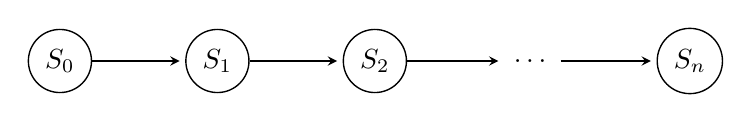
\begin{tikzpicture}[-> , >= stealth, shorten >=2pt, line width =0.5 pt,
        node distance=2 cm]
            \node [circle, draw] (zero) {$S_0$};
            \node [circle, draw, right of=zero] (one) {$S_1$};
            \node [circle, draw, right of=one] (two) {$S_2$};
            \node [right of=two] (dots) {$\dots$};
            \node [circle, draw, right of=dots] (n) {$S_n$};

            \path (zero) edge (one);
            \path (one) edge (two);
            \path (two) edge (dots);
            \path (dots) edge (n);
        \end{tikzpicture}
    \end{center}

    Formally, 
    \[[S_{n+1} \; | \; S_n, S_{n-1}, \dots, S_1] = [S_{n+1} \; | \; ]\]

    \textbf{Example (Simple Random Walk):} $S_{n+1} = S_n + X_{n+1}$ where $\P(X_{n+1} = \pm 1) = \frac{1}{2}$ 
    
    \textbf{Example:} Take a coin with $\P(H) = p, \; \P(T) = q$. What is the expected number of tosses until the pattern HHT appears? 

    We can draw a Markov chain for a particular pattern: 

    \begin{center}
        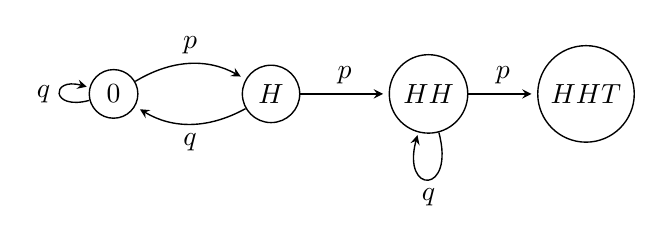
\begin{tikzpicture}[-> , >= stealth, shorten >=2pt, line width =0.5 pt,
        node distance=2 cm]
            \node [circle, draw] (zero) {$0$};
            \node [circle, draw, right of=zero] (H) {$H$};
            \node [circle, draw, right of=H] (HH) {$HH$};
            \node [circle, draw, right of=HH] (HHT) {$HHT$};

            \path (zero) edge [loop left] node {$q$} (zero);

            \path (zero) edge [bend left] node[above] {$p$} (H);
            \path (H) edge [bend left] node[below] {$q$} (zero);

            \path (H) edge node[above] {$p$} (HH);
            \path (HH) edge [loop below] node {$q$} (HH);

            \path (HH) edge node[above] {$p$} (HHT);

        \end{tikzpicture}
    \end{center}

\section{Oct 04}
\subsection*{Background}
    \textbf{Recall:} A Markov chain is a sequence of random variables $\{X_n\}_{n=0}^{\infty}$ such that
    \[\P(X_{n+1} \in A\; | \; X_{n} = x_n, \dots, X_0 = x_0) = \P(X_{n+1} \in A \; | \; X_n = x_n)\] 

    \textbf{State space:} Let $\S$ be all the possible values of $X_n$. In this class, assume $\S$ is countable.
    
    \textbf{Transition probability:} If $\P(X_{n+1} = y \; | \; X_n = x)$ is time-invariant (does not depend on $n$), then we call it \textbf{homogeneous} and write 
    \[P_{xy} = \P(X_{n+1} = y \; | \; X_n = x)\]

    \textbf{Transition matrix:} We can enumerate all the transition probabilities by 
    \[[P_{xy}]_{xy} = \begin{bmatrix}
        P_{00} & P_{01} & \dots\\
        P_{10} & P_{11} & \dots\\
        \vdots & \vdots & \ddots
    \end{bmatrix}\]
    which will have two very nice properties:
    \begin{enumerate}
        \item $P_{xy} \geq 0$ for all $x, y \in \S$
        \item $\sum_{y \in \S} P_{xy} = 1$ for all $x \in \S$ (each row sums to 1)
    \end{enumerate}

    \textbf{Example (Simple Random Walk):} Consider
    \[S_{n+1} = S_n + X_{n+1}\]
    over $\S = \Z$ where $\P(X_{n+1} = 1) = p$ and $\P(X_{n+1} = -1) = q$.

    Clearly, 
    \[\begin{cases}
        P_{x, x+ 1} = p\\ 
        P_{x, x-1} = q\\
        P_{x, y} = 0 & \text{ if } y\neq x \pm1 
    \end{cases}\]

\subsection*{Computational Problems}
    \textbf{Example:} 
    \begin{center}
        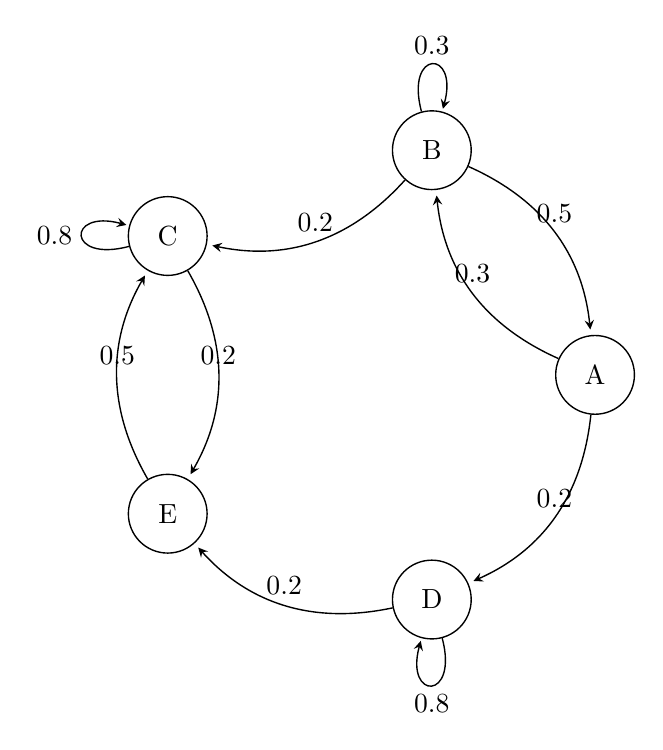
\begin{tikzpicture}[-> , >= stealth, shorten >=2pt, line width =0.5 pt]
            % Define the radius of the circle
            \def\radius{3cm}
            % Define the positions of the circles
            \foreach \i in {1,...,5} {
                \node[circle, draw, minimum size=1cm] (C\i) at ({360/5 * (\i - 1)}:\radius) {};
            }
            % Label the circles
            \node at (C1) {A};
            \node at (C2) {B};
            \node at (C3) {C};
            \node at (C4) {E};
            \node at (C5) {D};

            % Paths 
            \draw (C1) edge[bend left] node[above]{0.3} (C2); % A -> B
            \draw (C2) edge[bend left] node[above]{0.5} (C1); % B -> A
            \draw (C1) edge[bend left] node[above]{0.2} (C5); % A -> D
            \draw (C2) edge[loop above] node{0.3} (C2); % B -> B
            \draw (C2) edge[bend left] node[above]{0.2} (C3); % B -> C
            \draw (C3) edge[bend left] node[above]{0.2} (C4); % C -> E
            \draw (C3) edge[loop left] node{0.8} (C3); % C -> C
            \draw (C4) edge[bend left] node[above]{0.5} (C3); % E -> C 
            \draw (C5) edge[bend left] node[above]{0.2} (C4); % D -> E 
            \draw (C5) edge[loop below] node{0.8} (C5); % D -> D
        \end{tikzpicture}
    \end{center}

    So, for example, 
    \begin{itemize}
        \item $P_{AD} = 0.2$
        \item $P_{EA} = 0.5$
        \item $P_{ED} = 0$
    \end{itemize}

    \emph{Question 1:} What is the probability that starting from state $B$, the Markov Chain will hit state $D$ eventually

    Let's try first step analysis. Call $x_B$ the probability of hitting $D$ starting from $B$. 
    
    Then the first transition is just the probability of transitioning times the probability of hitting $D$ from the new state:
    \begin{align*}
        x_B &= P_{BA} x_A + P_{BB} x_B + P_{BC} x_C + P_{BD} x_D + P_{BE} x_E\\ 
        &= 0.5x_A + 0.3x_B + 0.2x_C 
    \end{align*}
    and if we repeat this for all states, we get a system of 5 linear equations with 5 unknowns -- which we can solve with a matrix!

    And to make things simpler, $x_D = 1$.

    And after finding all the equations and solving, we get $\boxed{x_B = 1}$

    \emph{Question 2:} What is the probability that starting from state $B$, the Markov Chain will hit state $D$ before state $E$?

    Again call this probability $x_B$ and notice that $x_s$ for $s \in \S$ is exactly the same as before (except with two special condition):
    \begin{itemize}
        \item $x_D = 1$
        \item $x_E = 0$
    \end{itemize}

    \emph{Question 3:} What is the average number of steps to reach state $D$ from state $A$? 

    We can once again call this $x_A$ and define 
    \[\begin{cases}
        x_s = 0 & \text{if } s = D\\
        x_s = P_{sA} (1 + x_A) + P_{sB} (1 + x_B) + P_{sC} (1 + x_C) + P_{sD} (1 + x_D) + P_{sE} (1 + x_E) & \text{otherwise}
    \end{cases}\]
    for $s \in \S$.

    \emph{Question 4:} Suppose the initial state is $A$. Let $T$ be the number of steps to reach $D$. In Q3, we calculated $\E[T]$. Now calculate 
    \[\E\left[\sum_{n=0}^{T-1} \beta^n \phi(x_n) \right]\]
    where $\phi(n)$ represent a payoff table 
    \begin{center}
        \begin{tabular}{c|c}
            $s$ & $\phi(x_S)$\\ 
            \hline
            A & 1\\ 
            B & 2\\ 
            C & 0\\ 
            D & -1\\ 
            E & 4            
        \end{tabular}
    \end{center}
    and $\beta$ is a discounting factor $0 < \beta < 1$.

    As always, let 
    \[x_A = \E\left[\sum_{n=0}^{T-1} \beta^n \phi(x_n) \right]\]
    
    How do we generalize to all states? 
    
    Once again we have special case $x_D = 0$. Now consider $x_A$. On the first step, we reach $A$ with probability $P_{AA}$ and the payoff will be $(\phi(A) + \beta x_A)$ so 
    \begin{align*}
        x_A &= P_{AA} (\phi(A) + \beta x_A)\\ 
        &\qquad + P_{AB}(\phi(A) + \beta x_B)\\ 
        &\vdots 
        &\qquad + P_{AE}(\phi(A) + \beta x_E)
    \end{align*}
    and analogously for all other states.

\section{Oct 07}
    \textbf{Example:} Let's see a case where first step analysis fails: 

    Let $S_{n+1} = S_n + X_{n+1}$ with $\P(X_{n+1} = 1) = p$ and $\P(X_{n+1} = -1) = q$ and $p> q$.

    \begin{center}
        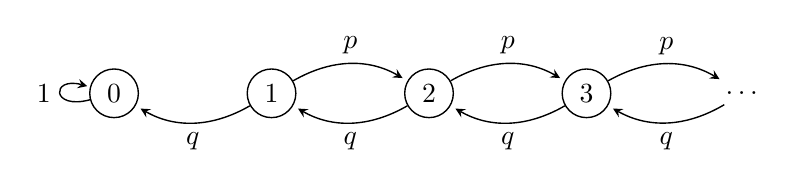
\begin{tikzpicture}[-> , >= stealth, shorten >=2pt, line width =0.5 pt,
        node distance=2 cm]
            \node [circle, draw] (zero) {$0$};
            \node [circle, draw, right of=zero] (one) {$1$};
            \node [circle, draw, right of=one] (two) {$2$};
            \node [circle, draw, right of=two] (three) {$3$};
            \node [right of=three] (dots) {$\dots$};
            
            \path (zero) edge[loop left] node[left]{$1$} (zero); 
            \path (one) edge[bend left] node[below]{$q$} (zero);
            \path (one) edge[bend left] node[above]{$p$} (two);
            \path (two) edge[bend left] node[below]{$q$} (one);
            \path (two) edge[bend left] node[above]{$p$} (three);
            \path (three) edge[bend left] node[below]{$q$} (two);
            \path (three) edge[bend left] node[above]{$p$} (dots);
            \path (dots) edge[bend left] node[below]{$q$} (three);
        \end{tikzpicture}
    \end{center}

    What is the probability $x_k$ that the random walk reaches $0$ eventually given that $S_0 = k$ and assuming $p > q$. 
    
    From first-step analysis, 
    \[x_k = px_{k+1} + qx_{k-1}\]
    for all $k \geq 1$ with $x_0 = 1$. 

    The characteristic equation is $r^2 = pr^2 + q \implies r = \{1, \frac{q}{p}\}$ 

    So the general solution is 
    \[x_k = Ar_1^k + Br_2^k = A + B \left(\frac{q}{p}\right)^k\]
    where $A, B$ are constants. 

    Plugging in the boundary condition, $A + B = 1$ so 
    \[x_k = 1 + B\left[\left(\frac{q}{p}\right)^k - 1\right]\] 

    But clearly, $0 \leq x_k \leq 1$ so $0 \leq B \leq 1$. But now $B$ cannot be uniquely determined -- \emph{every} such $B$ satisfies the boundary condition. What do we do now? 

    \emph{Option 1:} Artificially fix a large number $N$ and consider the $\{x_k\}_0^N$. The solution to the difference equation using first-step analysis will depend on $N$ so just let $N \to \infty$ and obtain $x_k$.

    \emph{Option 2:} Observe that (heuristically) $x_k \to 0$ as $k \to \infty$. (Rigorous follows from $p > q$ and some work).

    In either approach, we find $B = 1$ and 
    \[x_k = \left(\frac{q}{p}\right)^k\] 

    Both options work but both require some model-specific information which is not ideal. 

    Let's try to find a way to fix the first step analysis to determine the unique solution. 

    Consider a Markov chain with state space $\S$ and transition matrix $P$. Let $A \sub S$. 

    We define the \emph{hitting time} of $A$ as 
    \[T^A = \inf\{n \geq 0: X_n \in A\}\]
    with the convention that $\inf \emptyset = \infty$. 

    We want 
    \begin{align*}
        h^A(x) &= \P^x(T^A < \infty), 
        d^A(x) = \E^x[T^A]
    \end{align*}

    \begin{tbox}{\textbf{Theorem:} The vector $\{h^A(x): x \in \S\}$ is the minimal nonnegative solution of 
        \[h(x) = \begin{cases}
            \sum_{y \in \S} P_{xy}h(y) & x \notin A\\ 
            1 & x \in A
        \end{cases}\]
        Similarly, $\{d^A(x): x \in \S\}$ is the minimal nonnegative solution of
        \[d(x) = \begin{cases}
            1 + \sum_{y \in \S} P_{xy} h(y) & x \notin A\\
            0 & x \in A
        \end{cases}\]}

        \emph{Proof:} By the LTP, $\{h^A(x): x \in \S\}$ is certainly a solution. Now suppose $\{h(x): x \in \S\}$ is an arbitrary nonnegative solution. 

        We want to show that $h(x) \geq h^A(x)$ for all $x \in \S$. 

        If $x \in A$, $h(x) = h^A(x) = 1$. So choose $x \notin A$. 

        Repeatedly applying the system of equations, we get:
        \begin{align*}
            h(x) &= \sum_{y \in \S} P_{xy} h(y)\\ 
                &= \sum_{y \in A} P_{xy} h(y) + \sum_{y \notin A} P_{xy} h(y)\\ 
                &= \sum_{y \in A} P_{xy} + \sum_{y \notin A} P_{xy} \left[\sum_{z \in A} P_{yz} + \sum_{z \notin A} P_{yz} h(z)\right]\\
                &= \sum_{y \in A} P_{xy} + \sum_{y \notin A} \sum_{z \in A} P_{xy} P_{yz} + \sum_{y \notin A} \sum_{z \notin A} P_{xy} P_{yz} h(z)\\
                &= P^x(T^A = 1) + P^x(T^A = 2) + \sum_{y \notin A} \sum_{z \notin A} P_{xy} P_{yz} h(z)\\ 
                &\vdots
        \end{align*}

        So 
        \[h(x) \geq \P^x(T^A \leq n)\]
        for all $n$. Letting $n \to \infty$, we get 
        \[h(x) \geq \P^x(T^A < \infty) = h^A(x)\]

        For $\{d^A(x)\}$, by the tower property of conditional expectation, it is a solution to the corresponding system of equations. We take $\{d(x): x \in \S\}$ to be an arbitrary nonnegative solution and want to show that $d(x) \geq d^A(x)$. 

        Again $x \in A$ is trivial and for $x \notin A$, 
        \begin{align*}
            d(x) &= 1 + \sum_{y\notin A} P_{xy} d(y)\\ 
            &= 1 + P_{xy} \left[1 + \sum_{z \notin A} P_{yz}h(z)\right]\\ 
            &= P^x(T^A \geq 1) + P^x(T^A \geq 2) + \sum_{y\notin A} \sum_{z \notin A} P_{xy} P_{yz} d(z) 
        \end{align*}

        So, for all $N$, 
        \[d(x) \geq \sum_{n=1}^{N} P^x(T^A \geq n)\]

        And as $n \to \infty$, we know $T^A$ takes values in $\{0, 1, 2, \dots\} \cup \{\infty\}$ so 
        \[\sum_{n=1}^{\infty} \ind_{\{T^A\geq n\}} = T^A\]
        and taking the expectation of both sides, we are done. 
    \end{tbox}

    \textbf{Example:} Consider the MC $X$ with state space $\S = \{0, 1, 2, \dots\}$. Assume $P_{00} = 1$ and for all $x > 0$, 
    \[P_{xy} = \begin{cases}
        1/2 & y= 0\\ 
        1/4 & y = x + 1\\ 
        1/4 & y = x - 1\\ 
        0 & \text{otherwise}
    \end{cases}\] 
    modelled by 
    
   \begin{center}
   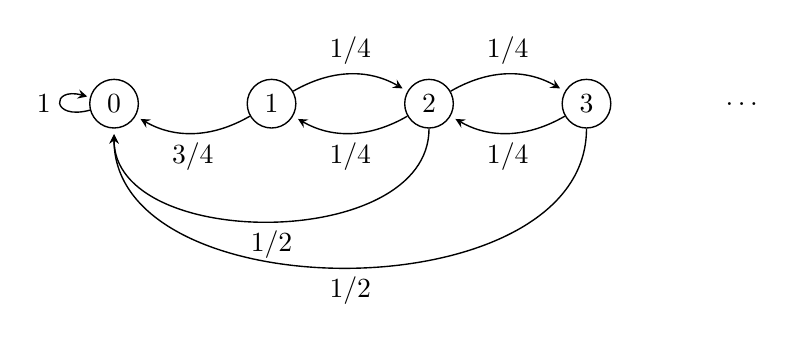
\begin{tikzpicture}[-> , >= stealth, shorten >=2pt, line width =0.5 pt,
    node distance=2 cm]
        \node [circle, draw] (zero) {$ 0 $};
        \node [circle, draw, right of=zero] (one) {$ 1 $};
        \node [circle, draw, right of=one] (two) {$ 2 $};
        \node [circle, draw, right of=two] (three) {$ 3 $};
        \node [right of=three] (dots) {$\dots$};
    
        \path (zero) edge[loop left] node[left]{$1$} (zero); 

        \path (one) edge[bend left] node[above]{$1/4$} (two);
        \path (two) edge[bend left] node[above]{$1/4$} (three);

        \path (one) edge[bend left] node[below]{$3/4$} (zero);
        \path (two) edge[bend left] node[below]{$1/4$} (one);
        \path (three) edge[bend left] node[below]{$1/4$} (two);

        \draw (two) edge[bend left=90] node[below]{$1/2$} (zero);
        \draw (three) edge[bend left=90] node[below]{$1/2$} (zero);
   \end{tikzpicture}
   \end{center}
    
    Let $T = \inf\{n \geq 0: X_n = 0\}$. We are interested in the average duration $d(x) = \E^x[T]$

    By the Theorem, $\{d(x): x \in \S\}$ is the minimal nonnegative solution to
    \begin{align*}
        d(x) &= 1 + \frac{1}{2}d(0) + \frac{1}{4}d(x + 1) + \frac{1}{4}d(x - 1)\\ 
        &= 1 + \frac{1}{4}d(x + 1) + \frac{1}{4}d(x - 1)
    \end{align*}
    for $x \geq 1$ with $d(0) = 0$. 

    If we consider $x$ an index, these equations are just a difference equation! (Excepting the ``1'' term which make it no longer homogeneous). 
    
    This allows us to follow the standard approach:
    \begin{enumerate}
        \item Find a particular sequence, ignoring the boundary condition. 
        
        Here, $d_p(x) = 2$

        \item FInd the general solution. 
        
        Here, $d_g(x) = d(x) - d_p(x)$ satisfies 
        \[d_g(x) = \frac{1}{4}d_{s}(x + 1) + \frac{1}{4}d_s(x - 1)\] 

        So $r = \frac{1}{4}r^2 + \frac{1}{4} \implies r = 2 \pm \sqrt{3}$ and 
        \[d_g(x) = Ar_1^x + Br_2^x = A(2 + \sqrt{3})^x + B(2 - \sqrt{3})^x\] 
        for constants $A, B$

        3. Fit the boundary condition. 

        Here, $d(x) = d_g(x) + d_p(x)$ with $d(0) = 0$ so $A + B = -2$ and 
        \[d(x) = A\left[(2 + \sqrt 3)^x - (2 - \sqrt 3)^x\right] + 2\left[1 - (2 - \sqrt 3)^x\right]\]

        Since $d(x)$ is nonnegative, $A \geq 0$ and the minimality of $d$ implies $A = 0$ so 
        \[d(x) = 2[1 -(2 - \sqrt 3)^x]\] 
    \end{enumerate}

    \textbf{Example (Branching Process):} Consider a stochastic model for population growth. Let $X_n$ denote the size of the population in the $n$-th generation. 

    Each individual independently reproduces a random number of offspring:
    \[X_{n+1} = \sum_{i=1}^{X_n} Z_i^{(n)} \]
    where $\{Z_i^{(n)}\}$ are iid with distribution 
    \[\P(Z = k) = p_k, \quad k = 0, 1, 2, \dots, \quad \sum_{k=0}^\infty p_k = 1\] 

    Assume $X_0 = 1$ and let $T = \ind\{n \geq 0: X_n = 0\}$ be the time to extinction. We are interested in $\P(T < \infty)$ (will the population ever go extinct?)

    Define for each $x \geq 0$, 
    \[H(x) = P^x(T_0 < \infty)\]
    which is the probability of extinction given initial population $x$. We want $\pi = H(1)$. 

    Again be the theorem, $\{H(x): x \geq 0\}$ is the minimal nonnegative solution to 
    \[H(x) = \sum_{k=0}^\infty P_{xk} H(x)\]
    for $x \geq 1$ with $H(0) = 1$, where $P_{xk} = \P(X_{n+1} = k \; | \; X_n = x)$ is the transition probability. 

    The key observation is that this system can be reduced to a single equation:
    \[H(x) = [H(1)]^x = \pi^x\]

    Therefore, we expect $\pi$ to satisfy 
    \[\pi = \sum_{k=0}^\infty P_{1k} \pi^k = \sum_{k=0}^\infty P_{k}\pi^k = \phi(\pi) \tag{*}\]

    And $\forall \pi$ that satisfy the above, 
    \[H(x) = \pi^x = \left[\sum_{i=0}^\infty P_i \pi^i\right]^x = \sum_{k=0}^\infty P_{xk} \pi^k = \sum_{k=0}^\infty P_{xk} H(k)\] 
    for $x \geq 0$ where the coefficient of $\pi^k$ is the sum of all possible ways to have $k$ offspring in total. Therefore, $\pi$ must be the guaranteed minimal solution.
    
    To solve $(*)$, we need to study $\phi$. 
    \begin{align*}
        \phi(0) = p_0\\ 
        \phi(1) = 1\\ 
        \phi'(0) = p_1\\ 
        \phi'(1) = \sum_{k=0}^\infty kp_k = \E[Z]
    \end{align*}
    so $\phi$ is increasing and convex. 
    
    Excluding the trivial case $p_0 = 0$ (the population will never go extinct), we assume $p_0 > 0$. 

    And with some calculus, 
    \begin{enumerate}
        \item If $p_0 > 0$ and $\E[Z] \leq 1$, then $\pi = 1$
        \item If $p_0 > 0$ and $\E[Z] > 1$, then $0 < \pi < 1$ 
    \end{enumerate}

    To give a numerical example, assume $p_k = p(1- p)^k$ for $k \geq 0$ where $p \in (0, 1)$ is a constant. This is equivalent to $Z +1$ be geometrically distributed with parameter $p$ so 
    \begin{align*}
        \E[Z] &= \frac{1}{p} - 1,\\ 
        \phi(\pi) &= \sum_{k=0}^\infty p(1- p)^k \pi^k\\ 
        &= \frac{p}{1 - (1 - p)\pi}
    \end{align*}
    
    $\pi = \phi(\pi)$ has two roots, $\{1, \frac{p}{1 - p}\}$ 

    Therefore, if $p \geq 1/2$ (or equivalently $\E[Z]\leq 1$), we have $\pi_1 \leq \pi_2$ and $\pi = 1$. On the other hand, if $p < 1/2$ (or $\E[Z] > 1)$, $\pi_1 > \pi_2$ and $\pi = \pi_2 < 1$

\section{Oct 09}
    \textbf{Recall (Branching Process):} 1st step analysis gives us the \emph{hitting probability} which guarantees a minimal nonnegative solution. 

    Take the case of a population where each member has a random number of offspring $Z$ where $\P(Z = 0) = p_0, \P(Z = 1) = p_1, \dots$. 

    We can define $\pi$ to be the probability of extinction. Clearly, 
    \begin{align*}
        \pi &= \sum_{k=0}^\infty \P(Z = k)\pi^k\\ 
            &= p_0 + p_1\pi + p_2\pi^2 + \dots\\ 
            &= \phi(\pi)
    \end{align*}

    This is called a \textbf{moment generating function}. 
    
    We have $\phi(0) = p_0$ and $\phi(1) = 1$. We can show that $\phi$ is increasing and convex.

    And then we can show that if $\phi'(1) < 1$, then $\phi$ has a solution less than $\pi = 1$ (a minimal solution). Otherwise, $\phi(1)$ is the minimal solution.

    Let's calculate. 
    \begin{align*}
        \phi'(\pi) &= p_1 + 2p_2 \pi + 3p_3\pi^2 + \dots\\
        \phi'(1) &= p_1 + 2p_2 + 3p_3 + \dots\\ 
            &= \E[Z]
    \end{align*}
    so 
    $\phi'(1) > 1 \iff \E[Z] > 1$. Hence, the probability the population goes extinct depends on the expected number of offspring (not surprising!)

    Now suppose $Z + 1$ is geometric with parameter $p$. Then
    \begin{align*}
        \P(Z = 0) &= p\\ 
        \P(Z = 1) &= pq\\ 
        \P(Z = 2) &= pq^2\\
        &\vdots
    \end{align*}
    where $q = (1 - p)$ and $0 < p < 1$. 

    So 
    \begin{align*}
        \phi(\pi) &= p + pq\pi + pq^2\pi^2 + \dots\\ 
            &= p\left(1 + q\pi + (q\pi)^2 + (q\pi)^3 + \dots\right)\\ 
            &= \frac{p}{1 - q\pi}
    \end{align*}
    
    $\pi = \frac{p}{1 - q\pi}$ is a quadratic with two roots: $\pi = \{1, \; \frac{p}{q}\}$. 

    Therefore, 
    \[\pi_2 < 1 \iff o< q \iff p < \frac{1}{2} \iff \E[Z + 1] = \frac{1}{p} > Z \iff \E[Z] > 1\]
    exactly as before. 

\subsection*{Martingales}
    \textbf{Martingale:} A stochastic process that on average stays constant 

    \textbf{Example (Random Walk):} 
    \[\begin{cases}
        S_0 = x\\ 
        S_{n+1} = S_n + X_{n+1}
    \end{cases} \iff S_{n+1} = x + \sum_{k=1}^{n+1} X_{n+1} \]
    where $X_n$ are iid R.V. with (say) $\P(X_n = \pm 1) = \frac{1}{2}$ 

    But 
    \[\E[S_{n+1} \; | \; S_n, S_{n-1}, \dots, S_0] = \E[S_{n+1} \; | \; S_n] = S_n\]
    so $S_n$ is a martingale.

    \textbf{Definition:} With
    \begin{enumerate}
        \item $\F_n= (Z_0, Z_1, \dots, Z_n)$ a is a \emph{filtration process} (reference) containing the information up to time $n$ for $Z = \{Z_0, Z_1, \dots\}$.
        \item $\{X_0, X_1, \dots\}$ is \emph{adapted} to $Z$, i.e. $X_n = X_n(Z_0, Z_1, \dots, Z_n)$
    \end{enumerate}
    then $\{X_n\}$ is a \textbf{martingale} (with respect to $Z$) if 
    \[\E[X_{n+1} \; | \; \F_n] = X_n\] 

    \textbf{Example:} 

    \begin{center}
    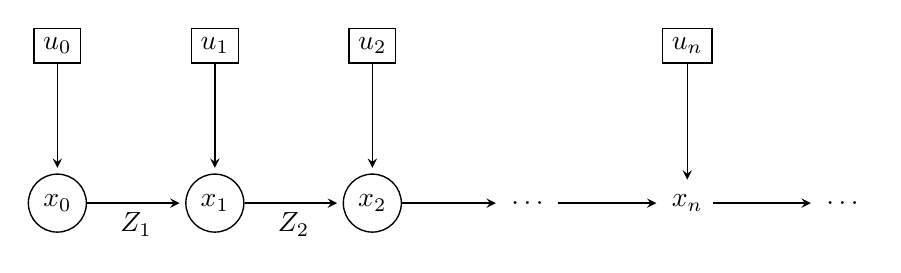
\begin{tikzpicture}[-> , >= stealth, shorten >=2pt, line width =0.5 pt,
    node distance=2 cm]
        \node [circle, draw] (zero) {$ x_0 $};
        \node [circle, draw, right of=zero] (one) {$ x_1 $};
        \node [circle, draw, right of=one] (two) {$ x_2 $};
        \node [right of=two] (dots) {$\dots$};
        \node [right of=dots] (n) {$ x_n $};
        \node [right of=n] (dots2) {$\dots$};

        \path (zero) edge node[below]{$Z_1$} (one);
        \path (one) edge node[below]{$Z_2$} (two);
        \path (two) edge (dots);
        \path (dots) edge (n);
        \path (n) edge (dots2);
    
        \node [rectangle, draw, above of=zero] (u0) {$ u_0 $};
        \node [rectangle, draw, above of=one] (u1) {$ u_1 $};
        \node [rectangle, draw, above of=two] (u2) {$ u_2 $};
        \node [rectangle, draw, above of=n] (un) {$ u_n $};

        \path (u0) edge (zero); 
        \path (u1) edge (one);
        \path (u2) edge (two);
        \path (un) edge (n);
    \end{tikzpicture}
    \end{center}

    So 
    \[X_{n+1} = f(X_n, u_n, Z_{n+1})\] 
    and we call $\{X_n\}$ a \emph{Markov Controlled Process}

    \textbf{Example:} Let $S_n$ be the standard random walk ($S_{n+1} = x_0 + \sum_{k=1}^{n+1} X_k$) such that $X_n$ are iid with $\E[X_n] = \mu$. 

    Define $Y_n = S_n - n \mu$. We claim $(Y_n)$ is a Martingale W.R.T $(X_n)$: 
    \begin{align*}
        \E[Y_{n+1} \; | \; \F_n] &= \E[S_{n+1} - (n + 1)\mu \; | \; \F_n]\\ 
        &= \E[S_{n+1} \; | \; \F_n] - (n + 1)\mu\\
        &= \E[S_n + X_{n+1} \; | \; \F_n] - (n + 1)\mu\\
        &= \E[S_n \; | \; \F_n] + \E[X_{n+1} \; | \; \F_n] - (n + 1)\mu\\
        &= \E[S_n \; | \; \F_n] + \mu - (n + 1)\mu\\
        &= S_n + \mu - (n + 1)\mu\\ 
        &= S_n - n\mu\\ 
        &= Y_n
    \end{align*}

\section{Oct 11}
    \textbf{Example (Wald's Martingale):} Let $X = \{X_0, X_1, \dots\}$ be a sequence of iid random variables and $\theta \in \R$ a constant. Let $\phi(\theta) = \E[e^{\theta X_1}]$ (the moment generating function) and 
    \[S_n = x_0 + \sum_{i=1}^{n} X_i \]
    for some $x_0 \in \R$ and all $n \geq 0$. Then the process 
    \[M_n = \frac{1}{\phi^n(\theta)} e^{\theta S_n}\]
    is a martingale with respect to the reference process $\{X_0, X_1, \dots\}$. It is not hard to verify this claim. 

    The adaptiveness is trivial and 
    \[\E[M_{n+1} \; | \; \F_n] = \frac{1}{\phi^{n+1}(\theta)} \E[e^{\theta S_{n+1}} \; | \; \F_n] = \frac{1}{\phi^{n+1}(\theta)} e^{\theta S_n} \E[e^{\theta X_{n+1}} \; | \; \F_n]\]

    Since $X_{n+1}$ is independent of $\F_n = (X_0, X_1, \dots, X_n)$ and has the same distribution as $X_1$, we have 
    \[\E[e^{\theta X_{n+1}} \; | \; \F_n] = \E[e^{\theta X_{n+1}}] = \E[e^{\theta X_1}] = \phi(\theta)\]

    Therefore, $\E[M_{n+1} \; | \; \F_n] = F_n$ and $\{M_n\}$ is a martingale. 

    \textbf{Example (Martingale Transform):} Let $M = \{M_0, M_1, M_2, \dots\}$ be a martingale with respect to some reference process $\{Z_0, Z_1, \dots\}$. Let $Y = \{Y_1, Y_2, \dots\}$ be a process such that $Y_n$ is a function of $\F_{n-1}$ for all $n \geq 1$ (such processes are said to be \emph{predictable}). 

    Define 
    \[X_n = \sum_{i=1}^{n} Y_i(M_i - M_{i-1}) = (Y \bullet M)_n \]
    for all $n\geq 0$. Then $\{X_n\}$ is a martingale with $X_0 = 0$. 

    The verification is not hard: The adaptiveness is trivial and 
    \begin{align*}
        \E[X_{n+1} \; | \; \F_n] &= X_{n+1} + \E[Y_{n+1}(M_{n+1} - M_n) \; | \; \F_n]\\
        &= X_{n+1} + Y_{n+1} \E[M_{n+1} - M_n \; | \; \F_n]\\
        &= X_{n+1}
    \end{align*}

    Note that the predictability of $Y$ is the only reason we can take $Y_{n+1}$ outside the conditional expectation. 

    In general, this procedure generates many martingales from a given martingale. Moreover, this is indeed a preliminary version of stochastic integral if $M_{n+1} - M_n$ is viewed as the differential $dM$ of the martingale $M$.

\subsection*{Optional Sampling}
    \textbf{Stopping time:} Let $Z = \{Z_0, Z_1, Z_2, \dots\}$ be a reference process. A mapping $\tau: \Omega \to \{0, 1, 2, \dots\} \cup \{\infty\}$ is said to be a \emph{stopping time} if for every $n$, the indicator random variable $\ind_{\tau = n}$ is a function of $\F_n = (Z_0, Z_1, \dots, Z_n)$. 
    
    Heuristically, the decision to stop at time $\tau$ is a stopping time iff the decision is based only on historical information. 

    \textbf{Example:} Let $X = \{X_n\}$ be adapted WRT $Z$ and $a \in \R$ constant. Define 
    \[\tau = \inf\{n \geq 0: X_n \geq a\}, \quad \sigma = \sup\{n\geq 0: Xn \geq a\}\]

    Both are random times but $\tau$ is a stopping time while $\sigma$ is not.

    \begin{tbox}{\textbf{Optional Sampling Theorem:} Let $X = \{X_0, X_1, \dots\}$ be a martingale and $\tau$ an arbitrary stopping time. Then 
        \[E[X_{\tau \land n}] = \E[X_0]\]
        for every $n$. If $X$ is a supermartingale or submartingale, then the equality is replaced by $\leq$ or $\geq$ respectively.}
        \emph{Proof:} We will only present the martingale case as the others are similar.

        Fix $n \geq 0$. Then 
        \[X_{\tau \land (n+1)} = X_{\tau} \ind_{\tau \leq n} + X_{n+1} \ind_{\tau > n}\]

        The key observation is 
        \[\ind_{\tau > n} = 1 - \ind_{\tau \leq n}\] 
        is a function of $\F_n$. Therefore, 
        \[\E[X_{n+1} \ind_{\tau > n} \; | \; \F_n] = \ind_{\tau > n} \E[X_{n+1} \; | \; \F_n] = \ind_{\tau > n} X_n\]

        By the tower property, taking expectation on both sides we have 
        \[\E[X_{n+1} \ind_{\tau > n}] = \E[X_n \ind_{\tau > n}]\]

        In particular, 
        \[\E[X_{\tau \land (n+1)}] = \E[X_{\tau} \ind_{\tau \leq n}] + \E[X_{n+1} \ind_{\tau > n}] = \E[X_{\tau \land n}]\]

        Since this is true for all $n$, the claim follows readily as $\tau \land 0 = 0$. 
    \end{tbox}

    \textbf{Remark:} Ideally, we would have $\E[X_{\tau}] = \E[X_0]$ when $X$ is a martingale in the Optional Sampling Theorem. However, one cannot hope this to be true in general. For example, let $X$ be a symmetric simple random walk and $\tau = \inf\{n \geq 0: X_n = 1\}$. Then $\E[X_{\tau}] = 1$ while $\E[X_0] = 0$.

    Therefore, we add conditions to ensure the $\E[X_{\tau}] = \E[X_0]$:
    \begin{enumerate}
        \item The stopping time is bounded, i.e. $\P(\tau \leq t) = 1$ for some $t \in \N$
        \item The process $\{X_n\}$ is bounded for $n = 1, \dots, \tau$
    \end{enumerate}

    In this course, some examples will not satisfy these conditions but it can nonetheless be shown that $\E[X_{\tau}] = \E[X_0]$. As we are not interested in rigor, \emph{assume that the equality holds if $X$ is a martingale and $\tau$ is a stopping time}.

\section{Oct 16}
    \tbf{Definition:}
    \begin{itemize}
        \item If $\E[X_{n+1} \; | \; \F_n] = X_n$, we say the process is a martingale 
        \item If $\E[X_{n+1} \; | \; \F_n] \leq X_n$, we say the process is a supermartingale
        \item If $\E[X_{n+1} \; | \; \F_n] \geq X_n$, we say the process is a submartingale
    \end{itemize}

    Further, using the Law of total expectation, $\E[\E[X_{n+1} \; | \; \F_n]] = \E[X_{n+1} \; | \; \F_n]$ so 
    \[\begin{cases}
        \E[X_{n+1}] = \E[X_n] & \text{ if martingale}\\
        \E[X_{n+1}] \geq \E[X_n] & \text{ if submartingale}\\ 
        \E[X_{n+1}] \leq \E[X_n] & \text{ if supermartingale} 
    \end{cases}\]

    \tbf{Recall (Optional Sampling Theorem):} If $(X_0, X_1, \dots)$ is a martingale and $\tau$ is a stopping time, 
    \[\E[X_{\tau \land n}] = \E[X_0] \quad \forall n\] 
    And under some conditions, 
    \[\E[X] = \lim_{n \to \infty} \E[X_{\tau \land n}] = \E[X_{\tau}]\]

    Specifically, these equalities hold if
    \begin{enumerate}
        \item if $\tau$ is bounded, i.e. $\P(\tau \leq N) = 1$ for fixed $N \in \N$.
        \item if $(X_n)$ is bounded on $n = 1, \dots, \tau$
    \end{enumerate}
    
    \textbf{Example (Gambler's Ruin):} Let $X = \{X_0, X_1, \dots\}$ be iid RVs with 
    \begin{align*}
        \P(X_1 = 1) &= p\\
        \P(X_1 = -1) &= q = 1 - p
    \end{align*}
    for $p \in (0, 1)$. One can think of $X_n$ as the net winning of a gambler at the $n$-th round. The gambler starts with \$ $x$ and he will leave if he reaches \$ $0$ or \$ $N$ for $0 < x < N$. The wealth process is 
    \[S_n = x + \sum_{i=1}^{n} X_i, \quad n \geq 0 \]

    From now on, we will let $\{X_n\}$ be the reference process. Then $S = \{S_0, S_1, \dots\}$ is adapted. Define the stopping time 
    \[\tau = \inf\{n \geq 0: S_n \in \{0, N\}\}\]

    We are interested in $\P(S_{\tau} = 0)$. 

    \begin{itemize}
        \item CASE 1: $p = q$. 
        
        The wealth process is a martingale itself. By the Optional Sampling Theorem, 
        \[\E[S_{\tau}] = \E[S_0] = x\] 

        And $0 \leq S \leq N$ until the game ends (Condition 2) but $S_{\tau} \in \{0, N\}$ so 
        \[x = \E[S_{\tau}] = N\P(S_{\tau} = N)\] 

        It follows that 
        \[\P(S_{\tau} =0 ) = 1 - \P(S_{\tau} = N) = 1 - \frac{x}{N} = \frac{N - x}{N}\]

        \item CASE 2: $p \neq q$. 
        
        Now the wealth process is not a martingale. Consider Wald's Martingale 
        \[M_n = \frac{1}{\phi^n(\theta)} e^{\theta S_n}\]
        for fixed $\theta$ and $n \geq 0$ where 
        \[e^{\theta x} = \E[M_0] = \E[M_{\tau}] = \E\left[\frac{1}{\phi^{\tau}(\theta)}e^{\theta S_{\tau}}\right]\]

        However now $\phi^{\tau}(\theta)$ cannot be taken outside the expectation. Since $\theta$ is arbitrary, choose $\theta$ such that $\phi(\theta) = 1$, i.e. $\theta \in \{0, \log(p/q)\}$. With $\theta = 0$, we have a constant martingale,  which is useless. 

        Therefore, let $\theta = \log(q/p)$ so 
        \[M_n = \left(\frac{q}{p}\right)^{S_n} \]
        is a martingale and 
        \begin{align*}
            \left(\frac{q}{p}\right)^x &= \E[M_0] = \E[M_{\tau}] = \E\left[\left(\frac{q}{p}\right)^{S_{\tau}} \right]\\ 
            &= \P(S_{\tau} = 0) + \left(\frac{q}{p}\right)^N \P(S_{\tau} = \left(\frac{q}{p}\right)^N)
        \end{align*}

        And $\P(S_{\tau} = 0) + \P(S_{\tau} = N) = 1$ so 
        \[\P(S_{\tau} = 0) = \frac{(q/p)^x - (q/p)^N}{1 - (q/p)^N}\]

        \textbf{Remark:} notice $1 < M_n < (q/p)^N$ up to time $\tau$ so we have again satisfied Condition 2.
    \end{itemize}

    We can define analogous OST for sub and supermartingales:
    \begin{itemize}
        \item Submartingale: $\E[X_{\tau \land n}] \geq \E[X_0]$
        \item Supermartingale: $\E[X_{\tau \land n}] \leq \E[X_0]$
    \end{itemize}

    \subsection*{Stochastic Optimization}
        There are two main branches in Stochastic Optimization:
        \begin{enumerate}
            \item Optimal Stopping (e.g. Secretary Problem)
            \item Optimal Control (e.g. utility maximization, Kelly criterion)
        \end{enumerate}

        Let's solve some of them with Martingales. 

        \tbf{Optimal Stopping (Finite Horizon):} Let $(X_0, X_1, \dots)$ be some process and $N$ a fixed terminal time. 
        \[V(x) = \max_{0 \leq \tau \leq N} \E\left[H(X_{\tau}) + \sum_{k=1}^{\tau-1} G(X_k) \;\bigg\vert X_0 = x\right]\]
        where $H(X_{\tau})$ is a terminal cost and $\sum_{k=1}^{\tau-1} G(X_k)$ is a running cost. 

        We can define this recursively
        \[V_n(x) =\max_{0 \leq \tau \leq N} \E\left[H(X_{\tau}) + \sum_{k=1}^{\tau-1} G(X_k) \;\bigg\vert S_n = x\right] \]
        so our DPE is 
        \[\begin{cases}
            V_n(x) = \max\left(H(x), \E[G(x) + V_{n+1}(X_{n+1}) \; | \; X_n = x]\right)\\ 
            V_N(x) = H(x)
        \end{cases}\]

\section{Oct 18}
\subsection*{Optimal Stopping (Finite Horizon)}
    Let $(X_0, X_1, \, \dots)$ a Markov chain with $P_{xy}$ transition matrix. 
    
    \[V(x) = \max\left(H(x), E^x[G(x) + V_{n+1}(X_{n+1})]\right)\]
    where $N$ is a fixed terminal time, $\tau$ is a stopping time, and $E^x$ is the expectation given $X_0 = x$.

    \begin{center}
    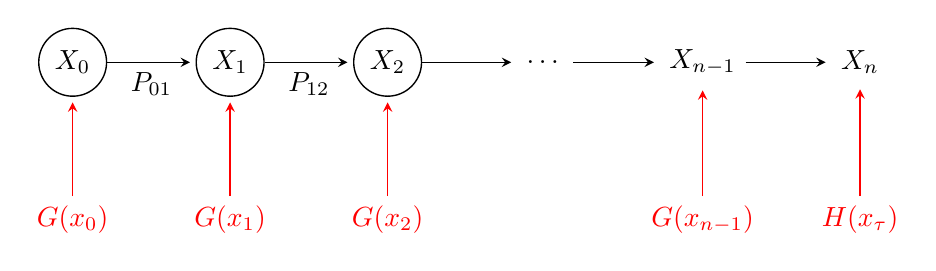
\begin{tikzpicture}[-> , >= stealth, shorten >=2pt, line width =0.5 pt,
    node distance=2 cm]
        \node [circle, draw] (zero) {$ X_0 $};
        \node [circle, draw, right of=zero] (one) {$ X_1 $};
        \node [circle, draw, right of=one] (two) {$ X_2 $};
        \node [right of=two] (dots) {$\dots$};
        \node [right of=dots] (n1) {$ X_{n-1} $};
        \node [right of=n1] (n) {$ X_n $};

    
        \path (zero) edge node[below]{$P_{01}$} (one);
        \path (one) edge node[below]{$P_{12}$} (two);
        \path (two) edge (dots);
        \path (dots) edge (n1);
        \path (n1) edge (n);
        
        \node[red, below of=zero] (G0) {$G(x_0)$};
        \node[red, below of=one] (G1) {$G(x_1)$};
        \node[red, below of=two] (G2) {$G(x_2)$};
        \node[red, below of=n1] (Gn1) {$G(x_{n-1})$};
        \node[red, below of=n] (Gn) {$H(x_{\tau})$};
        
        \path (G0) edge[red] (zero);
        \path (G1) edge[red] (one);
        \path (G2) edge[red] (two);
        \path (Gn1) edge[red] (n1);
        \path (Gn) edge[red] (n);
    \end{tikzpicture}
    \end{center}

    We can define value functions 
    \[V_n(x) = \max_{n \leq \tau \leq N} \E\left[H(x_{\tau}) + \sum_{k=n}^{\tau - 1} G(x_k) \bigg\vert X_n = x\right]\] 
    for all $0 \leq n \leq N$ and all $x$ with $V(x) = V_0(x)$. 

    At time $n$ with $X_n = x$, we can 
    \begin{enumerate}
        \item Stop, with payoff $H(x)$
        \item Continue, with payoff 
        \[G(x) + \E[V_{n+1}(x_{n+1}) \;|\; X_n = x] = G(x) + \sum_y P_{xy} V_{n+1}(y) \]
    \end{enumerate}
    where $G(x)$ is the payoff at time $n$ and $V_{n+1}(y)$ is the optimal payoff for $n+1$ given $X_{n+1} = y$.

    Hence, our DPE is
    \[\begin{cases}
        V_n(x) = \max\left\{H(x), G(x) + \sum_y P_{xy} V_{n+1}(y)\right\}\\ 
        V_N(x) = H(x)
    \end{cases}\]

    At last, we are ready to justify DP. 

    \begin{tbox}{\textbf{Theorem:} Suppose $\{v_0(x), v_1(x), \dots, v_N(x)\}$ is a solution to the DPE. Then $v_n(x) = V_n(x)$ for all $n$. Moreover, define $\tau^* = \inf \{n \geq 0: V_n(x) = H(x)\}$. Then $\tau^*$ is an optimal stopping time.}
        \emph{Proof:} Define 
        \[M_n = \sum_{k=0}^{n- 1} G(x_k) + v_n(x_n)\]
        that is, $M_n$ is a Markov Chain which behaves optimally for $m \geq n$. 

        We claim that $\{M_n\}$ is a supermartingale. 
        \begin{align*}
            \E[M_{n+1} \; | \; \F_n] &= \E\left[\sum_{k=0}^{n} G(x_k) + v_{n+1}(x_n) \; | \; \F_n\right]\\
            &= \sum_{k=0}^n G(x_k) + \E[v_{n+1}(x_{n+1}) \; | \; \F_n] \qquad \qquad (x_{0:n} \in \F_n)\\
            &= \sum_{k=0}^n G(x_k) + \E[v_{n+1}(x_{n+1}) \; | \; x_n] \qquad\qquad (\text{Markov property}) \\
            &= \sum_{k=0}^{n-1} G(x_k) + G(x_n) + \E[v_{n+1}(x_{n+1}) \; | \; x_n]\\
            &\leq \sum_{k=0}^{n-1} G(x_k) + v_n(x_n) \hspace{1in} (\text{DPE})\\
            &= M_n
        \end{align*}

        Then, by the Optional Sampling Theorem, for any $0\leq \tau \leq N$, $\E[M_{\tau}] \leq \E[M_0]$. 

        Therefore, 
        \[\E\left[\sum_{k=0}^{\tau - 1} G(x_k) + v_{\tau}(x_{\tau})\right] \leq v_0(x_0)\]

        But in the DPE, clearly $v_n(x) \geq H(x)$ for all $n$ so 
        \begin{align*}
            \E\left[\sum_{k=0}^{\tau - 1} G(x_k) + H(x_{\tau})\right] &\leq \E\left[\sum_{k=0}^{\tau - 1} G(x_k) + v_{\tau}(x_{\tau})\right]\\ 
                &\leq v_0(x_0) 
        \end{align*}
        and
        \[v_0(x_0 \geq V_0(x))\]

        But if $\tau^* = \inf\{n \geq 0: v_n(x) = H(x)\}$, then clearly $v_{\tau^*}(x_{\tau^*}) = H(x_{\tau^*})$ so 
        \[\E\left[\sum_{k=0}^{\tau - 1} G(x_k) + H(x_{\tau})\right] = \E\left[\sum_{k=0}^{\tau - 1} G(x_k) + v_{\tau}(x_{\tau})\right]\] 

        Finally, for $n < \tau^*$, $v_n(x_n) \neq H(x_n)$ so $v_n(x_n) = G(x_n) + \E[v_{n+1}(x_{n+1}) \; | \; x_n]$ so 
        \[\sum{k=0}^{n-1} G(x_k) + v_{\tau^*}(x_{\tau^*}) = v_0(x_0)\]
        and $M_n$ is a martingale. 
    \end{tbox}

\section*{Oct 21}
    \tbf{Recall:} For Finite Horizon Optimal Stopping problems, we have 
    \[V(x) = \max_{0 \leq \tau \leq N} \E\left[\int_{x_0}^x H(x_{\tau}) + \sum_{k=0}^{\tau - 1} G(X_k) \right]\] 
    for $\tau^* = \min\{n \geq 0: v_n(x_n) = H(x_n)\}$. 

    We can write a DPE 
    \[\begin{cases}
        v_N(x) = H(x)\\ 
        \begin{aligned}
            v_n(x)&= \max_{n \leq \tau \leq n} \E[H(x_{\tau}) + \sum_{k=n}^{\tau - 1} G(x_k)\; | \; x_n = x]\\ 
            &= \max\left\{H(x), G(x) + \sum_y P_{xy} v_{n+1}(y)\right\}
        \end{aligned}
    \end{cases}\]

\subsection*{Optimal Stopping (Infinite Horizon)} 
    In infinite horizon case, the setup is very similar:
    \[V(x) = \max_{0 \leq \tau} \E\left[H(x_{\tau}) + \sum_{k=0}^{\tau - 1} G(x_k)\right]\]
    and we have DPE 
    \[v(x) = \max\{H(x), G(x) + \sum_y P_{xy} v(y)\} \tag{*}\]

    But! This no longer has a unique solution. Let's use the finite horizon version to help. 

    Define $u_n(x) = v_{N - n}(x)$ (or equivalently $u_{N -n } = v_n(x)$) where $N$ is the terminal time from the finite horizon case. 
    
    Now we are indexing by ``time to go'' so we have a \emph{forward form DPE}:
    \[\begin{cases}
        u_0(x) = H(x)\\ 
        u_{n+1}(x) = \max\{H(x), G(x) + \sum_y u_n(y) P_{xy}\}
    \end{cases}\]
    which gives us $\{u_0, u_1, \dots, u_N\}$ 

    Intuitively, we expect $u_n(x) \to V(x)$ as $n \to \infty$. Taking the limit, 
    \[V(x) = \min\{H(x), G(x) + \sum_y V(y) P{xy}\}\]

    So now it remains to show that $V(x)$ is indeed the minimal solution to the DPE. 

    \begin{tbox}{\textbf{Proposition:} $V(x)$ is the minimal solution to the DPE }
        \emph{Proof Sketch:} 
        \begin{enumerate}
            \item $V(x) = \lim_{n \to\infty} u_n(x)$
            \item Suppose there is another solution $u(x)$. WTS $u(x) \geq V(x)$. 

            But from (*), 
            \begin{align*}
                u(x) &\geq H(x) = u_0(x)\\ 
                u(x) &\geq G(x) + \sum_y P_{xy} u(y)\\ 
                    &\geq G(x) + \sum_y P_{xy} u_0(y)
            \end{align*}
            so 
            \[u(x) \geq \max\{H(x), G(x) + \sum_y P{xy} u_1(y)\} = u_2(x)\] 
            and we can inductively verify that $u(x) \geq u_n(x)$ for all $n$.
    
            Hence, $u(x) \geq \lim u_n(x) = V(x)$
        \end{enumerate}
    \end{tbox}

\subsection*{Optimal Control}
    In a control problem, $X_{n+1} = f(x_n, u_n, \xi_{n+1})$ where $u_n$ is the control at time $n$ and $\xi_{n+1}$ is the noise at time $n+1$.

    We can model it as a Markov Chain 
    \begin{center}
    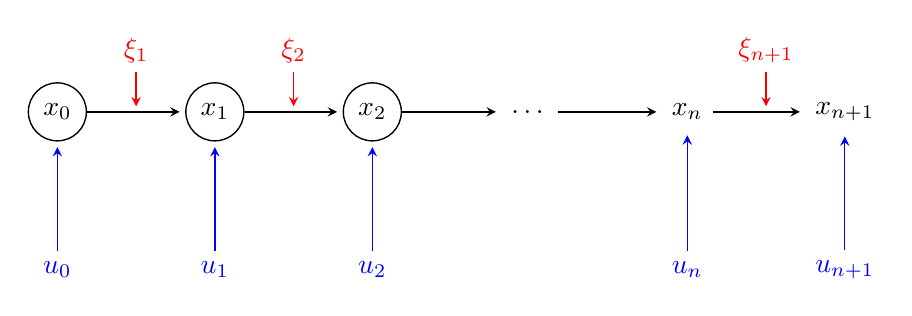
\begin{tikzpicture}[-> , >= stealth, shorten >=2pt, line width =0.5 pt,
    node distance=2 cm]
        \node [circle, draw] (zero) {$ x_0 $};
        \node [circle, draw, right of=zero] (one) {$ x_1 $};
        \node [circle, draw, right of=one] (two) {$ x_2 $};
        \node [right of=two] (dots) {$\dots$};
        \node [right of=dots] (n) {$ x_n $};
        \node [right of=n] (n1) {$x_{n+1}$};
    
        \path (zero) edge (one);
        \path (one) edge (two);
        \path (two) edge (dots);
        \path (dots) edge (n);
        \path (n) edge (n1);

        \node [below of=zero, blue] (u0) {$u_0$};
        \node [below of=one, blue] (u1) {$u_1$};
        \node [below of=two, blue] (u2) {$u_2$};
        \node [below of=n, blue] (un) {$u_n$};
        \node [below of=n1, blue] (un1) {$u_{n+1}$};

        \path (u0) edge[blue] (zero);
        \path (u1) edge[blue] (one);
        \path (u2) edge[blue] (two);
        \path (un) edge[blue] (n);
        \path (un1) edge[blue] (n1);

        \node [red, above=0.5cm of $(zero)!0.5!(one)$] (z1) {$\xi_1$};
        \node [red, above=0.5cm of $(one)!0.5!(two)$] (z2) {$\xi_2$};
        \node [red, above=0.5cm of $(n)!0.5!(n1)$] (zn1) {$\xi_{n+1}$};

        \path (z1) edge[red] ($(zero)!0.5!(one)$);
        \path (z2) edge[red] ($(one)!0.5!(two)$);
        \path (zn1) edge[red] ($(n)!0.5!(n1)$);    
    \end{tikzpicture}
    \end{center}

    \tbf{Finite Horizon Optimal Control:}
    \[V(x) = \max_{\{u_n\}} \E\left[H(x_n) + \sum_{k=0}^{N-1} G(x_k, u_k) \;\bigg\vert\; x_0 = x \right]\]
    for terminal time $N$. 

    We can define value functions
    \[v_n(x) = \max_{\{u_k\}} \E[H(x_N) + \sum_{k=0}^{n-1} G(x_k, u_k) + v_{n+1}(x_{n+1}) \;\bigg\vert\; x_n = x]\]
    which yields DPE 
    \[\begin{cases}
        v_N(x) = H(x)\\ 
        v_n(x) = \max_{u \in A(x)} [G(x, u) + v_{n+1}(f(x, u, \xi_{n+1}))]
    \end{cases}\]

    \begin{tbox}{\textbf{Theorem:} $V(x) = v_0(x)$. And if $u_n^*(x) \in A_n$ is the maximizer to the RHS of the DPE, then $\{u_0^*(x), u_1^*(x), \dots\}$ is an optimal control policy}
        \emph{Proof:} Omitted (similar to earlier proofs)
    \end{tbox}

\section*{Oct 23}
\subsection*{Infinite Horizon Optimal Control:}
    \[V(x) = \max_{\{u_n\}} \E\left[\sum_{n=0}^\infty \alpha^n G(x_n, u_n) \; \bigg\vert \; x_0 = x \right]\]
    where $0 < \alpha < 1$ is a discount factor to make the sum convergent and $X_{n+1} = f(x_n, u_n, \xi_{n+1})$

    Notice 
    \begin{align*}
        \sum_{k=0}^\infty\alpha^k G(x_k, u_k) &= G(x_0, u_0) + \alpha \sum_{k=1}^\infty \alpha^{k} G(x_k, u_k)\\
        &= G(x_0, u_0) + \alpha \sum_{k=1}^\infty \alpha^{k-1} G(x_{k}, u_{k})\\
        &= G(x_0, u_0) + \alpha V(x)
    \end{align*}
    where $V(x)$ is the value if we control optimally.

    Then our DPE is 
    \begin{align*}
        V(x) &= E[G(x, u) + \alpha V(f(x, u, \xi))]\\ 
            &= \max_{u \in A(x)} \left\{G(x, u) + \alpha \E[V(f(x, u, \xi))]\right\}
    \end{align*}
    but because we have no terminal condition, we have no guarantee of a unique solution -- even when $G$ is continuous and bounded!
    
    How do we calculate the value function? By definition,
    \[\begin{cases}
        v_0(x) = 0\\ 
        v_{n+1}(x) = \max_{u \in A(x)} \left\{G(x, u) + \alpha \E[v_n(f(x, u, \xi))]\right\}
    \end{cases} \tag{*}\]
    Then clearly, if $v_n \to v^*$ then $v^*$ is a solution to the DPE.

    \begin{exercise}
        \textbf{Exercise:} Check that 
        \[v_n(x) = \max_{\{u_k\}} \E\left[\sum_{k=0}^{n-1} \alpha^k G(x_k, u_k) \; \bigg\vert \; x_0 = x\right]\]
        i.e. (*) is a forward DPE with unique solution
    \end{exercise}

\subsection*{Contraction Principle}

    In its most general form, we can think of a DPE as a \emph{functional} $v = \L(v)$. Then existence of a solution amounts to asking if $\L$ has a fixed point.

    For $v_0 = v$ (any initial condition), we define $v_n = \L(v_{n-1})$. It suffices to show that $v_n$ is Cauchy. Of course, this requires us to first define a metric on the space of functions: we will take the uniform metric 
    \[\rho(u, v) = \sup_x \abs{u(x) - v(x)}\]

    \tbf{Definition:} a space $(\F, \rho)$ of functions equipped with a metric $\rho$ is \emph{complete} if every Cauchy sequence in $\F$ has a limit in $\F$. 

    Let's return to the DPE: 
    \[v(x) = \max_{u \in A(x)} \left\{G(x, u) + \alpha \E[v(f(x, u, \xi))]\right\}\]

    Assume $G$ is bounded. Then $\L$ maps a bounded function to a bounded function. 

    \begin{exercise}
        \textbf{Exercise:} Show that the space of bounded functions is complete under the uniform metric.
    \end{exercise}

    \begin{tbox}{\textbf{Claim:} $\rho(\L(v), \L(w)) \leq \alpha \rho(v, w)$ for $0 < \alpha < 1$ }
        \emph{Proof:} 
        \begin{align*}
            \rho(\L(v), \L(w)) &= \sup_x \abs{\L(v)(x) - \L(w)(x)}\\
            &= \sup_x \bigg\vert\max_{u \in A(x)} \left\{G(x, u) + \alpha \E[v(f(x, u, \xi))]\right\}\\ 
                &\qquad - \max_{u \in A(x)} \left\{G(x, u) + \alpha \E[w(f(x, u, \xi))]\right\}\bigg\vert\\
            &= \alpha \sup_x \abs{\E[v(f(x, u, \xi))] - \E[v(f(x, u, \xi))]}
            &\leq \alpha \sup_x \abs{v(x) - w(x)}\\ 
            & = \alpha \rho(v, w)
        \end{align*}

        Hence, $\L$ is a contraction
    \end{tbox}

    \tbf{Claim:} for a contraction $\L$ and any initial function $v_0$, $v_n = \L(v_{n-1})$ is Cauchy
    
    \tbf{Claim:} if a contraction has a fixed point, it is unique.

    All together, $v_n$ is Cauchy and hence has a limit $v^*$ which is a fixed point of $\L$. Therefore, $v^*$ is a solution to the DPE.

\chapter{Dynamic Programming: Applications}
\section*{Oct 25}
\subsection*{Optimal Stopping on SRW with Absorbing End Points} 

    Let $\{S_0, S_1, S_2, \dots\}$ be a symmetric random walk with 
    \[S_n = S_0 + \sum_{k=1}^{n} X_k\] 
    until the walk is absorbed at $0$ or $b \in \N$, with $\{X_1, X_2, \dots\}$ iid with $\P(X_1 = 1) = \P(X_1 = -1) = 1/2$ and $S_0 = x \in \{0, 1, \dots, b\}$. 
    
    Let $f: \{0, 1, \dots, b\} \to [0, \infty)$. The goal is to solve 
    \[v(x) = \sup_{\tau} \E[f(S_{\tau}) \; | \; S_0 = x]\]
    where $\tau$ is the stopping time when the walk is absorbed.

    Clearly, $v$ is a solution to the DPE 
    \[V(x) = \max\{f(x), \frac{1}{2}V(x + 1) + \frac{1}{2}V(x  -1)\}, \quad 0 < x < b\]
    and we have boundary conditions $V(0) =0$, $V(b) = f(b)$.

    This DPE implies $v$ is concave and dominates $f$. Further, if $V(x) > f(x)$, we must have 
    \[V(x) = \frac{1}{2}V(x +1) + \frac{1}{2}V(x - 1)\] 
    so $V$ is linear at $x$. 

    With a little work, we can show that $V$ is in fact the \emph{smallest} concave function that dominates $f$ and that the optimal stopping time is 
    \[\tau^* = \inf\{n \geq 0: V(S_n) = f(S_n)\}\]

    An interesting special case is when $f(x) = \ind_{\{x = 0\}}$. Then it is never optimal to stop (stopping gives zero value) and instead continue until absorption, i.e. 
    \[\begin{cases}
        V(x) = (b - x) / b\\ 
        \tau^* = \inf\{n \geq 0: V(S_n = f(S_n))\} = \inf\{n \geq 0: S_n = 0 \text{ or } b\} 
    \end{cases}\]

    Moreover,
    \[\frac{b - x}{b} = V(x) = \P(S_{\tau^*} = 0 \; | \; S_0 = x) = \P(\text{random walk reaches 0 before b} \; | \; S_0 = x)\]
    which is the ruin probability for fair games. 

\subsection*{A Discounted Random Walk}
    Consider another symmetric SRW $\{S_0, S_1, S_2, \dots\}$ with 
    \[S_n = S_0 + \sum_{k=1}^{n} X_k\] 
    for $\{X_1, X_2, \dots\}$ iid with $\P(X_1 = 1) = \P(X_1 = -1) = 1/2$.

    Let $\alpha \in (0, 1)$ be a discount factor for the optimization problem 
    \[V(x) = \sup_{\tau} \E[\sum_{k=0}^{\tau - 1} \alpha^k S_k \; | \; S_0 = x]\]

    This is an infinite horizon discounted optimal stopping problem so the value function should satisfy the DPE 
    \[V(x) = \max\{0, x + \frac{\alpha}{2} [V(x + 1) + V(x - 1)]\}\]

    Let's try to solve it explicitly, for which we need a guess of the optimal stopping strategy. Notice that if $S_n$ is strictly positive, it is never optimal to stop since the RW will still be non-negative in the next step which will contribute positively to the expected value. Conversely, if $S_n$ is very negative we should cut our losses and stop:
    \[V(x) = \begin{cases}
        x + \frac{\alpha}{2} [V(x + 1) + V(x - 1)] & x > b\\ 
        0 & x \leq b
    \end{cases}\] 
    for $b$ a \emph{free-boundary} such that it is optimal to stop when $S_n \leq b$ and optimal to continue when $S_n > b$. 

    Note that for $x \geq b$, $V$ satisfies a difference equation with characteristic equation 
    \[r = \frac{\alpha}{2}(r^2 + 1)\]
    with roots $\frac{1}{\alpha}(1 \pm \sqrt{1 - \alpha^2})$ and particular solution $x/(1 - \alpha)$. 

    Therefore if $x \geq b$, 
    \[V(x) = \frac{x}{1 - \alpha} + A\left(\frac{1 - \sqrt{1 - \alpha^2}}{\alpha}\right)^x + B\left(\frac{1 - \sqrt{1 + \alpha^2}}{\alpha}\right)^x\]
    for constants $A, B$. 

    Solving the DPE thus reduces to determining the constants $A, B, b$. 

    \begin{enumerate}
        \item \emph{Determination of $B$}: It is not hard to verify $0 < r_1 < 1 < r_2$. But $V \geq 0$ and can grow at most linearly as $x \to \infty$ since 
        \[V(x) \leq \E[\sum_{k=0}^\infty \alpha^k \abs{S_k} \; | \; S_0 = x] \leq \sum_{k=0}^\infty \alpha^k(x + k)\]
        so $B = 0$.

        \item \emph{Determination of $A$:} Denote $r = \frac{1 - \sqrt{1 - \alpha^2}}{\alpha}$. By definition, $V(b) = 0$ so 
        \[V(b) = \frac{b}{1 - \alpha} + Ar^b = 0 \implies A = - \frac{br^{-b}}{1 - \alpha}\]
        and 
        \[V(x) = \begin{cases}
            \frac{1}{1 - \alpha} (x - br^{x - b}) & x \geq b\\ 
            0 & x \leq b
        \end{cases}\] 

        \item \emph{Determination of $b$:} For $x > b$, it is optimal to continue so we expect the value of continuation to be larger than the value of stopping:
        \[x + \frac{\alpha}{2}[V(x + 1) + V(x - 1)]\]
        for $x > b$.

        Conversely, for $x \leq b$, it is optimal to stop:
        \[x + \frac{\alpha}{2}[V(x + 1) + V(x - 1)] \leq 0\]

        Plugging $V$ into these inequalities, 
        \begin{align*}
            \frac{1}{1 - \alpha} (x - br^{x- b}) &> 0 && x > b\\ 
            b + \frac{\alpha}{2} \frac{1}{1 - \alpha} (b+ 1  -br) &\leq 0 && x = b\\ 
            x &\leq 0 && x < b
        \end{align*}

        But we expect $b \leq 0$ so the last inequality always holds. The LHS of the first case is increasing when $x \leq b$ so it reduces to $x = b + 1$. Therefore, the system reduces to 
        \[\begin{cases}
            \frac{1}{1 - \alpha} (x - br^{x- b}) > 0 & x = b + 1\\ 
            b + \frac{\alpha}{2} \frac{1}{1 - \alpha} (b+ 1  -br) \leq 0 & x = b
        \end{cases}\]

        Solving, we get 
        \begin{align*}
            D &= -\frac{1}{1 - r} < b\\ 
            C &= -\frac{\alpha}{2 - \alpha - \alpha r} \geq b
        \end{align*}
        and by definition of $r$, $C = D + 1$ so $b$ is the unique negative integer in 
        \[(D, D+1] = \left(-\frac{1}{1 - r}, -\frac{r}{1 - r}\right]\]

        This procedure also verifies that $V$ is indeed a solution to the DPE! 

    \end{enumerate}

\section*{Oct 28}
    \tbf{Remark:} It is very common in practice to solve entry and exit problems. But in general, solving
    \[\max_{\tau \leq 0} \E\left[\sum_{k=\tau}^{\sigma - 1} \alpha^k S_k \; | \; S_0 = x\right]\]
    and 
    \[\max_{\tau} \E\left[\alpha^{\tau} V(S_{\tau}) \; | \; S_0 = x\right]\]
    are equivalent. 

\subsection*{Search Problem}
    Let's consider a very general problem. 
    
    Let $\{X_0, X_1, \dots\} \geq 0$ be iid R.V. with density $f$. 

    We want to find 
    \[\max_{\tau} \E[\max(x_1, x_2, \dots, x_{\tau}) - c\tau]\]
    for $c > 0$ constant. 

    Our value function is just $V(x)$ for $x$ the current best offer. 

    And our DPE is
    \[V(x) = \max\left(x, \E[V(\max(x, X))] - c\right)\]
    where $x$ is our value of stopping and the other term is the value of continuation. 

    The optimal strategy is to find a threshold $x^*$ such that it is optimal to stop if $x \geq x^*$

    \begin{center}
        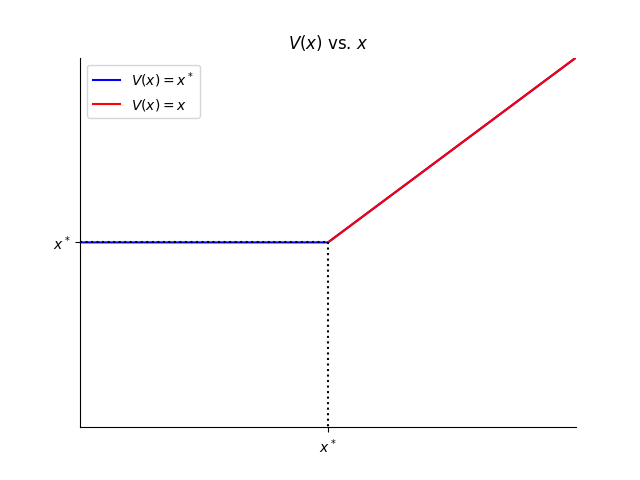
\includegraphics[width=0.8\textwidth]{Images/x_star search.png}
    \end{center}

    How do we determine $x^*$? 

    Notice, $\forall x < x^*$, $x^* = V(x) = \E[V(\max(x, X))] - c$ so for $X \sim f(y)$,
    \begin{align*}
        x^* &= \E[V(\max(x, X))] - c\\ 
            &= \int_0^{\infty} V(\max(x, u)) f(y)\; dy - c\\ 
            &= \int_0^{x^*} V(\max(x, y)) f(y)\; dy + \int_{x^*}^{\infty} V(\max(x, y)) f(y)\; dy - c\\ 
            &= \int_0^{x^*} x^* f(y)\; dy + \int_{x^*}^{\infty} y f(y)\; dy - c\\
            &= x^*
    \end{align*}

    Define $\phi(x) = \int_x^{\infty} (y - x) f(y)\; dy$ so $c = \phi(x^*)$ and $\phi \to 0$ from $\phi(0) = \E[X]$

\section{Oct 30}
\subsection*{Linear Regulator}
    Let $\{\zeta_1, \zeta_2, \dots\}$ be iid R.V. with mean $0$ and variance $\sigma^2$ (representing noise). The controlled process is given by 
    \[X_{n+1} = X_n - u_n + \zeta_{n+1}\]
    where $\{u_0, u_1, \dots\}$ is a sequence of controls in $\R$> 

    Given a discount factor $\alpha \in (0, 1)$ and a constant $\ep > 0$, we want to solve 
    \[V(x) = \inf_{\{u_n\}} \E\left[\sum_{n=0}^\infty \alpha^n (X_n^2 + \ep u_n^2)\; \bigg\vert \; X_0 = x\right]\]
    where the inf is taken over all possible controls. 

    Clearly, this should satisfy the DPE
    \[V(x) = \inf_u \{x^2 + \ep u^2 + \alpha \E[V(x - u + \zeta)]\}\]
    where $\zeta$ is drawn from the distribution of $\zeta_1$. 

    What form will the value function take? If we do a few iterations with the forward DPE of the corresponding finite horizon problem, we can see that $V$ will be quadratic in $x$. 

    Assume $V(x) = ax^2 + bx + c$ for constants $a, b, c$. Then
    \begin{align*}
        V(x) &= ax^2 + bx + c \\ 
        &= \inf_u \{x^2 + \ep u^2 + \alpha E(a(x - u + \zeta) + b(x - u + \zeta) + c)\}\\ 
        &= \inf_u \{x^2 + \ep u^2 + \alpha[a(x - u)^2 + a\sigma^2 + b(x - u) + c)\}\\
    \end{align*}
    which is minimized at 
    \[u = u^* = \frac{\alpha (2 ax + b)}{2(\ep + \alpha a)}\]
    
    Plugging this back in and comparing the coefficients for $x$, 
    \[b = \frac{\alpha b}{\ep + \alpha a} \implies b = 0\]
    and for $x^2$,
    \[a = 1 + \frac{\ep \alpha a}{\ep + \alpha a}, \quad c = \alpha(a \sigma^2 + c)\]

    Solving by noting that $a > 0$ so $V \geq 0$, 
    \[a = \frac{(\ep \alpha + \alpha  \ep)^2 + \sqrt{(\ep \alpha + \alpha - \ep)^2 +4\alpha \ep}}{2\alpha}, \quad c = \frac{\alpha\sigma^2}{1 - \alpha}a\]

    Therefore, $V(x) = ax^2 + c$ and the optimal control at time $n$ is 
    \[u_n^* = \frac{\alpha a}{\ep + \alpha a} X_n\]



\chapter{Brownian Motion and Stochastic Calculus}
\section{Nov 1}
    Consider the classical random walk. Let $\{X_1, X_2, \dots\}$ be iid R.V. with $\P(X_1 = 1) = \P(X_1 = -1) = 1/2$.

    These random variables satisfy $\E[X_i] = 0$ and $\Var[X_i] = 1$. The SRW associated with $\{X_i\}$ (starting at the origin) is 
    \[S_n = \sum_{i=1}^n X_i\]
    for $n\geq 0$.

    We want to approximate Brownian motion. Given large $n$, define 
    \[S^(n)(t) = \sum_{i=1}^{nt} X_i, \quad 0 \leq t \leq 1\] 
    which is a ``picture'' of the whole RW $\{S_0, S_1, \dots, S_n\}$ scaled down. 

    \tbf{Remark:} When we write $nt$ in the sum, we mean it is defined when $nt$ is an integer and as a linear interpolation between the two closest integers otherwise.

    But this time scaling is not enough to fully put the RW in a pcutre since $S^{(n)}$, the state of the RW, can take very large values. So how should be scale the state space?

    If we scale by a factor of $1/n$, the process is 
    \[\frac{1}{n} S^{(n)}(t) = \frac{1}{n}\sum_{i=1}^{nt} X_i\]
    which will be very close to a constant line of $0$ when $n$ is large (LLN). But this removes all the randomness! 

    Heuristically, we should choose $1/\sqrt{n}$ -- the factor consistent with the Central Limit Theorem. Therefore, define
    \[B^{(n)}(t) = \frac{1}{\sqrt n} \sum_{i=1}^{nt} X_i, \quad 0 \leq t \leq 1\]

    For $n$ large, we can already make some important observations:
    \begin{itemize}
        \item The process is continuous in $t$. (The jump sizes of the SRW are $1/\sqrt n \to 0$)
        \item The RV $B^{(n)}(t)$ is \emph{approximately} normal $N(0, t)$. (CLT)
        \item The increment $B^{(n)}(t) - B^{(n)}(s) \approx N(0, t - s)$ for $0 \leq s < t \leq 1$ (Proof: Exercise. Hint: CLT)
        \item We can trivially extend the definition for any $t \geq 0$. 
        \item All of the above are valid as long as $\E[X_i] = 0$ and $\Var[X_i] = 1$ 
    \end{itemize}

    Letting $n \to \infty$, we naturally get the definition of a Brownian motion.

    \tbf{Standard Brownian Motion:} A stochastic process $B = \{B(t): t \geq 0\}$ is a Brownian motion if:
    \begin{enumerate}
        \item $B_0 = 0$
        \item The sample path $t \mapsto B_t$ is always continuous
        \item The increment $B_t - B_s \sim N(0, t - s)$ for all $0 \leq s < t$
        \item The increments on disjoint time intervals $\{B_{t_1} - B_{t_0}, B_{t_2} - B_{t_1}, \dots, B_{t_n} - B_{t_{n-1}}\}$ are independent for all $n$ and $0 \leq t_0 \leq \dots \leq t_n$.
    \end{enumerate}

\subsection*{Interlude: Jointly Normal Random Variables}
    A jointly normal (multivariate normal) distribution of $n$ variables is characterized by 
    \begin{itemize}
        \item $\mu \in \R^n$ given by $\mu_k = \E[X_k]$ 
        \item $\Sigma \in \R^{n \times n}$ given by $\Sigma_{ij} = \Cov(X_i, X_j)$ (and $\Sigma_{ii} = \Var(X_i)$)
    \end{itemize}
    which gives us some very nice properties:
    \begin{enumerate}
        \item the covariance matrix $\Sigma$ is symmetric 
        \item Independent random variables are jointly normal \emph{automatically} 
        \item Any linear combination of a jointly normal distribution is normal (i.e $aX + bY \sim N$ if $X, Y \sim N$)
    \end{enumerate}

\subsection*{Properties of Standard Brownian Motion}
    Brownian motion is \emph{the} most fundamental stochastic process. From its definition we have some elementary properties:
        \begin{itemize}
            \item $B_t \sim N(0, t)$
            \item $\{B_{t_1}, B_{t_2}, \dots, B_{t_n}\}$ (given by $B_{t_i} = B_{t_i} - B_{t_{i-1}}$) is jointly normal. 
            
            In particular, for $s < t$, 
            \[X = aB_s + bB_t\] 
            ($a, b$ constant).

            We know
            \begin{align*}
                \E[X] &= a\E[B_s] + b\E[B_t] = 0\\ 
                \Var[X] &= \Var[aB_s + bB_t]\\ 
                    &= \Var(aB_s + b(B_s + (B_t - B_s)))\\ 
                    &= \Var((a + b) B_s + b(B_t - B_s))\\ 
                    &= \Var((a+ b) B_s) + \Var(b(B_t - B_s)) && (\text{independence})\\ 
                    &= (a + b)^2 s + b^2(t - s)
            \end{align*}
            so 
            \[X \sim N(0, (a^2 + 2ab)s + b^2t)\]
            
            \item For any $s < t$, $\Cov(B_s, B_t) = s$. In general, $\forall s, t$ we have $\Cov(B_s, B_t) = \min(s, t)$. 
            
            Say $s < t$. Then 
            \begin{align*}
                \Cov(B_s, B_t) &= \Cov(B_s, B_s + (B_t - B_s))\\ 
                & = \Cov(B_s, B_s) + \Cov(B_s, B_t - B-s) \\ 
                &= \Var(B_s) + 0
            \end{align*}
            since $B_s$ and $B_t - B_s$ are independent.
        \end{itemize}

\section{Nov 4}
\subsection{A second construction of Brownian Motion}
    \begin{tbox}{\textbf{Lemma:} Let $\{B_t: t \geq 0\}$ be a standard Brownian motion. For any $0 \leq s < t$ and  $c = (s + t)/2$,
    \[X = B_c - \frac{1}{2} (B_s + B_t) \sim N(0, \frac{t-S}{4})\]
    is independent of $(B_s, B_t)$. Indeed, $X$ is independent of $B_u$ for any $u \notin (s, t)$}
        \emph{Proof:} The RVs $(B_s, B_c, B_t)$ are jointly normal. Therefore $(X, B_s, B_t)$ are also jointly normal since they are linear combinations of jointly normal RVs. 

        We can compute 
        \begin{align*}
            \Cov(X, B_s) &= \Cov(B_c - B_s) - \frac{1}{2}(B_s, B_t) -\frac{1}{2}\Cov(B_t, B_s)\\ 
                &= s - \frac{s}{2} - \frac{t}{2} = 0\\ 
            \Cov(X, B_t) &= \Cov(B_c - B_t) - \frac{1}{2}\Cov(B_s, B_t) - \frac{1}{2}\Cov(B_t, B_t)\\
                &= t - \frac{s}{2} - \frac{t}{2} = 0
        \end{align*}

        Therefore, $X$ is independent of $B_s$ and $B_t$. Similarly, we can show that $\Cov(X, B_u) = 0$ for all $u \notin (s, t)$ and thus conclude that $X$ is independent of $B_u$ as well. 

        Moreover, $X$ is normal with mean $0$ and variance 
        \begin{align*}
            \Var\, X &= \Var\left[\frac{1}{2}(B_c - B_s) + \frac{1}{2}(B_c - B_t)\right]\\ 
                &= \frac{1}{4} (c - s) + \frac{1}{4}(t - c)\\ 
                &= \frac{t - s}{4}
        \end{align*}
    \end{tbox}

    It follows immediately from the lemma that for $0 \leq s < t$, one can represent $B_c$ as 
    \[B_c = \frac{B_s + B_t}{2} + \frac{\sqrt{t - s}}{2}Z\]
    where $Z \sim N(0, 1)$ is independent of $(B_s, B_t)$ and in general $B_u$ for all $u \notin (s, t)$. 

    Thus, Brownian motion is a ``linear'' combination of standard normal RVs. 

    Precisely, let $\{Z_1, Z_2, \dots\}$ be iid $N(0, 1)$ and consider $t \in [0, 1]$. 
    \begin{enumerate}
        \item \emph{First level approximation:} Define $B_0$ and $B_1 = Z_1$. Use linear interpolation for any $0  < t < 1$
        \item \emph{Second level approximation:} Let $c_1 = (0 + 1)/2$ and $\Delta_1 = 1 - 0$. Define 
        \[B_c = \frac{B_0 + B_1}{2} + \frac{\sqrt{\Delta_1}}{2} Z_2\]
        Use linear interpolation for any $0 < t < c$ and $c < t < 1$. 
        \item \emph{Third level approximation:} Let $c_2 = (0 + c_1)/2$ and $\Delta_2 = c_1 - 0$. Define
        \[B_{c_2}= \frac{B_0 + B_{c_1}}{2} + \frac{\sqrt{\Delta_2}}{2} Z_3\]
        use linear interpolation for any $0 < t < c_2$, $c_2 < t < c_1$. Deal with the time interval $(c_1, 1)$ analogously. 
    \end{enumerate}

    \begin{center}
        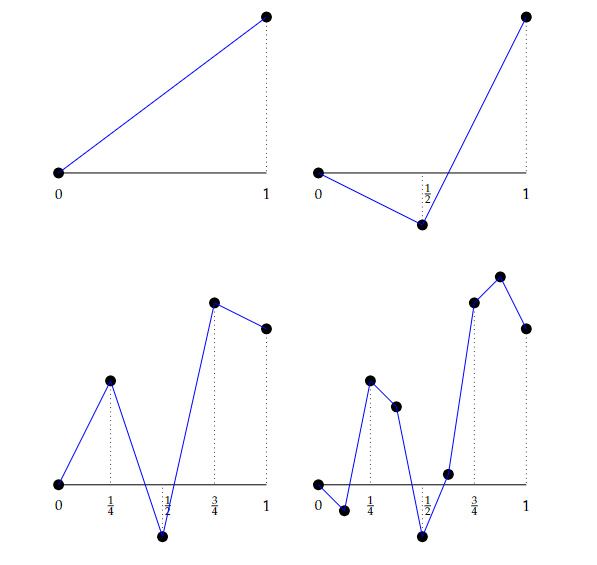
\includegraphics{Images/Brownian iteration.png}
    \end{center}

    If one is willing to sort out all the technical details, these approximations can be expressed as 
    \[B_t^{(m)} = \sum_{k=1}^{2^m} S_k^{(m)}(t) Z_k\] 
    for the $m^{\text{th}}$ level approximation, where $\{Z_1, Z_2, \dots\}$ are iid $N(0, 1)$ and $\{S_1^{(m)}, S_2^{(m)}, \dots\}$ are a family of functions on $[0, 1]$ with 
    \[S_k^{(m)}(t) = \int_0^t H_k^{(m)}(s)\; ds\] 
    where $\{H_k^{(m)}(t)\}$ form a complete orthonormal basis of $L^2[0, 1]$.

    We call $\{H_k^{(m)}\}$ the \emph{Haar wavelets}. They are rectangle shaped functions:

    \begin{center}
        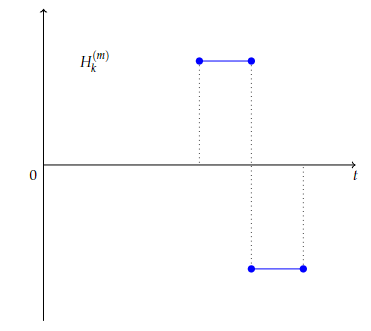
\includegraphics{Images/Haar wavelets.png}
    \end{center}

\subsection{Properties of Brownian Motion}
    Let $B = \{B_t: t \geq 0\}$ be a standard Brownian motion. It is straightforward from the definition that 
    \begin{itemize}
        \item (Symmetry) $-B = \{-B_t: t \geq 0\}$ is also a standard Brownian motion
        \item Brownian motion starts afresh at every time. That is, for any $s > 0$, $\{W_t = B_{t + s} - B_s: t \geq 0\}$ is a standard Brownian motion.
    \end{itemize} 

    \tbf{Example (Reflection Principle):} Let $B$ be a standard Brownian motion and $T > 0$ an arbitrarily fixed time. Define 
    \[M_T = \max\{B_t: 0 \leq t \leq T\}\]

    We would like to find the distribution of $M_T$. It is obvious that $M_T \geq 0$. Therefore, it suffices to calculate $\P(M_T > x)$ for any constant $x> 0$. Let 
    \[\sigma = \min\{t  \geq 0: B_t = x\}\]

    That is, $\sigma$ is the first time the Brownian motion reaches the level $x$. By definition, we must have $\{\sigma < T\} = \{M_T > x\}$. Therefore, 
    \[\P(M_T > x) = \P(\sigma < T)\]

    On the other hand, if $\{B_T > x\}$, then we must have $\{\sigma < T\}$. Therefore, 
    \[\P(B_T > x) = \P(B_T > x \land \sigma < T) = \P(B_T > x \; | \; \sigma  < T) \P(\sigma < T)\]

    The conditional probability in the preceding display must be $0.5$ by the symmetry of the standard Brownian motion and the reflection principle. Therefore,
    \[\P(B_T > x) = \frac{1}{2}\P(\sigma < T) = \frac{1}{2}\P(M_T > x)\]
    but $B_T \sim N(0, T)$. Thus, letting $\Phi$ be the CDF of $N(0, 1)$, 
    \[\P(M_T > x) = 2\P(B_T > x) = 2\P\left(N(0, 1) > \frac{x}{\sqrt T}\right) = 2\Phi\left(-\frac{x}{\sqrt T}\right)\]

    Taking the derivative WRT $x$, we get the density of $M_T$:
    \[\frac{2}{\sqrt T} \Phi'(-\frac{x}{\sqrt T}) \ind_{\{x\geq 0\}} = \frac{2}{\sqrt{2\pi T}} e^{-x^2/2T} \ind_{\{x \geq 0\}}\]

    \begin{center}
        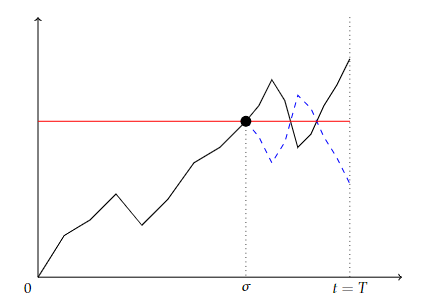
\includegraphics{Images/Reflection principle.png}
    \end{center}

\subsection{Martingales and Brownian Motion} 
    
    Recall in the definition of martingales that we have a reference process $\{Z_n\}$ and an adapted process $\{X_n\}$ that satisfies 
    \[\E[X_{n+1} \; | \; Z_0, Z_1, \dots, Z_n] = X_n\]

    With a little technical work, we can extend this notion to continuous time. In general, we can choose the Brownian motion $\{B_t: t \geq 0\}$ itself as the reference process. An adapted process $\{X_t: T \geq 0\}$ is a process such that for every $t \geq 0$, $X_t$ is a function of $\F_t = \{B_s: 0 \leq s < t\}$, the history of the Brownian motion up to time $t$.

    For example, $X_t = B_t^2 - t$ or $X_t = M$ are both adapted processes. A process $X = \{X_t\}$ is said to be a martingale WRT $B = \{B_t\}$ if $X$ is adapted to the reference process and $\E[X_{t+s} \; | \; \F_t] = X_t$ for all $s, t \geq 0$. 

    Many times we will simply say that $X$ is martingale when the underlying reference process $B = \{B_t: t \geq 0\}$ is obvious. Of course, one can define submartingales or supermartingales in the same way.

    Given a (reference process) standard Brownian motion $B= \{B_t\}$, there are many martingales. For example, it is easy to see that both $X_t = B_t$ and $X_t = B_t^2 - t$ are martingales.

    A slightly more complicated example is the \emph{exponential martingale} 
    \[X_t = e^{\theta B_t - \frac{1}{2} \theta^2 t}\]
    for any constant $\theta$. 

    It turns out that most stochastic integrals are indeed martingales (or close to being martingales if not). Theorems such as optional sampling theorem for discrete time carry over to continuous time. Let us work out a couple of simple examples.

    Define
    \[\sigma =  \min \{t \geq 0: B_t = -a \text{ or } B_t = b\}\]

    We would like to compute $\E[\sigma]$ and $\P(B_{\sigma} = -a)$. Consider the standard Brownian motion $B$ itself. Trivially, it is a martingale:
    \[\E[B_{t + s} \; | \; \F_t] = \E[B_t \; | \; \F_s] + \E[B_{t+s}  - B_t \; | \; \F_t] = B_t + \E[B_{t+s} - B_t] = 0\]
    (second equality follows from the independence of increments).

    Applying the optional sampling theorem,
    \[0 = \E[B_0] = \E[B_{\sigma}] = -a \P(B_{\sigma} = -a) + b \P(B_{\sigma} = b)\]
    But $B_{\sigma} \in \{-a, b\}$ so $\P(B_{\sigma} = -a) + \P(B_{\sigma} = b) = 1$. Therefore, 
    \[\P(B_{\sigma} = -a) = \frac{b}{a + b}\]

    Finally, consider the martingale $X_t = B_t^2 - t$. By the optional sampling theorem,
    \[0 = \E[X_0] = \E[X_{\sigma}] = \E[B_{\sigma}^2] - \E[\sigma]\]
    so 
    \[\E[\sigma] = \E[B_{\sigma}^2] = (-a)^2 \P(B_{\sigma} = -a) + b^2 \P(B_{\sigma} = b) = ab\]

    \tbf{Remark:} Brownian motion is a martingale but also a Markov process in the sense that given $\F_t$, the distribution of $\{B_s: s > t\}$ only depends on $B_t$. 

\section{Nov 8}
\section{Stochastic Integral}
    Throughout this section, we will implicitly assume that teh reference process is some standard Brownian motion $B = \{B_t: t \geq 0\}$. A classsical Riemann integral is of the form 
    \[\int_a^bf(x) \; dx\]
    representing the sum of infinitesimal increments. 
    
    A stochastic integral is of the form 
    \[\int_0^{T} X_t \; dB_t\]
    where $X = \{X_t\}$ is some adapted process. The difference is that for the latter, the increments are random variables. 

    Further, due to the properties of Brownian motion. \emph{the fundamental theorem of calculus does not hold for stochastic integrals}.

    \tbf{Example:} Consider 
    \[\int_0^a x\; dx, \qquad \int_0^T B_t \; dB_t\]

    \begin{itemize}
        \item \emph{Computation of the Riemann integral:} Fix a large $n$. Partition the interval $[0, a]$ into $n$ subintervals of length $a/n$. Then
        \[\int_0^a x\; dx = \lim_{n \to \infty} \sum_{i=0}^{n- 1} x_i \Delta x_i = \lim_{n \to \infty} \sum_{i=0}^{n- 1} x_i(x_{i+1} - x_i)\]
        where $x_i = i(a/n)$ so 
        \begin{align*}
            \lim_{n \to \infty} \sum_{i=0}^{n- 1} x_i (x_{i+1}- x_i) &= \lim_{n \to \infty} \sum_{i=0}^{n- 1} \left(\frac{x_{i+1} + x_i}{2} - \frac{x_{i+1} - x_i}{2}\right) (x_{i+1} - x_i)\\ 
            &= \lim_{n \to \infty} \left[\frac{1}{2}  \sum_{i=0}^{n- 1} (x_{i+1}^2 - x_i^2) - \frac{1}{2}\sum_{i=0}^{n- 1} (x_{i+1} - x_i)^2\right]\\ 
            &= \lim_{n \to \infty} \left[ \frac{a^2}{2} - \frac{1}{2}\sum_{i=0}^{n- 1} (\Delta x_i)^2\right]\\ 
            &= \lim_{n \to \infty} \left[ \frac{a^2}{2} - \frac{1}{2}\sum_{i=0}^{n- 1} \frac{a^2}{n^2}\right]\\ 
            &= \lim_{n \to \infty} \left[ \frac{a^2}{2} -\frac{a^2}{2n}\right]\\ 
            &= \frac{a^2}{2}
        \end{align*}

        \item \emph{Computation of the stochastic integral:} Divide the interval $[0, T]$ into $n$ subintervals of length $T/n$: $0 = t_0 <t_1 < \dots < t_n = T$ with $t_i = i(T/n)$ and $\Delta t_i = t_{i+1} - t_i = \frac{T}{n}$. 
        
        We define the stochastic integral as 
        \begin{align*}
            \lim_{n \to \infty} \sum_{i=0}^{n- 1} B_{t_i} (B_{t_{i+1}} - B_{t_i}) &= \lim_{n \to \infty} \sum_{i=0}^{n- 1} \left(\frac{B_{t_{i+1}} + B_{t_i}}{2} - \frac{B_{t_{i+1}} - B_{t_i}}{2}\right) (B_{t_{i+1}} - B_{t_i})\\
            &= \lim_{n \to \infty} \left[\frac{1}{2} \sum_{i=0}^{n- 1} (B_{t_{i+1}}^2 - B_{t_i}^2) - \frac{1}{2} \sum_{i=0}^{n- 1} (B_{t_{i+1}} - B_{t_i})^2\right]\\
            &= \frac{1}{2} B_t^2 \bigg\vert_0^T - \frac{1}{2} \sum_{i=0}^{n- 1}(B_{t_{i+1}} - B_{t_i})^2
        \end{align*}

        In the Riemann integral, this second term tends to 0. However, by the definition of Brownian motion, 
        \[B_{t_{i+1}} - B_{t_i} \sim N(0, t_{i+1} - t_i) = N(0, \frac{T}{n})\]

        It follows that $\sqrt{n}(B_{t_{i+1}}- B_{t_i})$ are iid $N(0, T)$ R.V. for $i =0, 1, 2, \dots, n -1$. Therefore, $n(B_{t_{i+1}} - B_{t_i})^2$ are iid random variabnles with expected value 
        \[E[n(B_{t_{i+1}} - B_{t_i})^2] = 0 + T = T\]

        So 
        \[\int_0^T B_t \; d B_t = \lim_{n \to \infty} \sum_{i=1}^{n-1} B_{t_i}(B_{t_{i+1}} - B_{t_i}) = \frac{1}{2}B_t^2 \bigg\vert_0^T - \frac{1}{2} T = \frac{1}{2}(B_T^2 - T)\]

        In short, the Fundamental Theorem of Calculus does not hold for stochastic integrals because Brownian motion simple paths have too much variation
    
    \end{itemize}

    
    \tbf{Definition:} Let $X = \{X_t\}$ be an adapted process and $T>0$ constant. We define the stochastic integral
    \[\int_0^T X_t \; dB_t = \lim_{n \to \infty} \sum_{i=0}^{n-1} X_{t_i} (B_{t_{i+1}} - B_{t_i})\]
    where $0 = t_0 < t_1 < t_2 < \dots < t_n = T$ is an arbitrary partition of $[0, T]$. 

    Obviously, we would like an analogous fundamental theorem for the stochastic integral. Consider a continuously differentiable function $f$ with anti-derivative $F$. We should consider the stochastic integral with $X_t = f(B_t)$:
    \[I_T = \int_0^T f(B_t)\; dB_t\]

    Fix an arbitrarily large $n$ and a fine partition $0 < t_0 < t_1 < \dots < t_n = T$. Then by definition, 
    \[I_T = \lim_{n \to \infty} \sum_{i=0}^{n-1} f(B_{t_i}) (B_{t_{i+1}} - B_{t_i}) = \lim_{n \to \infty} \sum_{i=1}^{n-1} F'(B_{t_i})(B_{t_{i+1}} - B_{t_i}) \]

    From the Taylor expansion, 
    \[F(x + \Delta x) - F(x) = F'(x) \Delta x + \frac{1}{2} F''(x) \Delta x^2 + O(\Delta x^3)\]

    It follows that 
    \[F'(B_{t_i})(B_{t_{i+1}} - B_{t_i}) = F(B_{t_{i+1}}) - F(B_{t_i}) - \frac{1}{2}F''(B_{t_i})(B_{t_{i+1}} - B_{t_i})^2 + O(\Delta x_i^3)\]
    and 
    \[\sum_{i=1}^{n-1} F'(B_{t_i})(B_{t_{i+1}} - B_{t_i}) = F(B_T) - F(B_0) - \frac{1}{2}\sum_{i=1}^{n-1} F''(B_{t_i})(B_{t_{i+1}} - B_{t_i})^2 + \sum_{i=0}^{n -1} O(\Delta x_i^3)\]

    While it is not true in general that $O(\Delta x_i^3) = 0$, we do have 
    \[\lim_{n \to \infty} \sum_{t=0}^{n-1} O(\Delta x_i^3) = 0\]

    This makes intuitive sense because $(B_{t_{i+1}} - B_{t_i})^3 \sim (\sqrt{\Delta t_i})^3 Z_i^3$ where $Z_i \sim N(0, 1)$. 

    They key development of stochastic calculus is the analysis of the summation in the middle of the RHS. In the example above, $F''(x)$ is just a constant and we can use LLN. In general, we need something stronger. 

    Recall $\Delta t_i = t_{i+1} - t_i$. We have 
    \[\sum_{i=1}^{n-1} (B_{t_{i+1}} - B_{t_i})^2 = \sum_{i=1}^{n-1} F''(B_{t_i}) \Delta t_i + \sum_{i=1}^{n-1} F''(B_{t_i}) \left[(B_{t_{i+1}} - B_{t_i})^2 - \Delta t_i\right]\]

    We claim that 
    \begin{align*}
        \sum_{i=1}^{n-1} F''(B_{t_i}) \Delta t_i &\overset{n \to \infty}{\longrightarrow} \int_0^T F''(B_t) \; dt\\ 
        Q_n = \sum_{i=1}^{n-1} F''(B_{t_i}) \left[(B_{t_{i+1}} - B_{t_i})^2 - \Delta t_i\right] &\overset{n \to \infty}{\longrightarrow} 0
    \end{align*}

    The first equation is obvious. The second is a bit more subtle. Recall that $B_{t_{i+1}} - B_{t_i} = \sqrt{\Delta t_i} Z_i$ where $Z_i \sim N(0, 1)$. Further, by the independenet increment property of Brownian motion, $Z_i$ is independent of 
    \[\{Z_0, Z_1, \dots, Z_{i-1}, F''(B_{t_0}), F''(B_{t_1}), \dots, F''(B_{t_{i-1}})\}\]

    Then all the cross terms have $0$ expected value so 
    \[\E[Q_n^2] = \sum_{i=1}^{n-1} \E[F''(B_{t_i}) (Z_i^2 - 1)\Delta t_i]^2 = C \sum_{i=1}^{n-1} \E[F''(B_{t_i})]^2 (\Delta t_i)^2 \to 0\]
    where $C = \E(Z_i^2 - 1)^2$. 

    All together, we get the \tbf{Itô Formula}:
    \begin{align*}
        \int_0^T F'(B_t) \; dB_t &= F(B_t)\bigg\vert_0^T - \frac{1}{2}\int_0^T F''(B_t) \; dt\\
        &= F(B_T) - F(B_0) - \frac{1}{2}\int_0^T F''(B_t) \; dt
    \end{align*}
    or equivalently, 
    \[F(B_T) = F(B_0) + \int_0^T F'(B_t) \; dB_t + \frac{1}{2}\int_0^T F''(B_t)\; dt\]

    Luckily, it is often not necessary to evaluate the stochastic integral directly.

    \begin{tbox}{\textbf{Theorem:} Let $X = \{X_t\}$ be an adapted process. THen the stochastic integral $\{I_t: t \geq 0\}$ defined by 
        \[I_t = \int_0^t X_s \; dB_s\] 
        is a martingale under mild conditions. In particular, its expected value is $0$.}
        \emph{Proof:} Exceedingly technical, hence omitted. 

        \emph{Heuristic Argument:} Fix any $T > 0$. Consider a partition $t_n$ of $[0, T]$. 

        We have 
        \begin{align*}
            I_T = \int_0^T X_t \; dB_t &\approx \sum_{i=0}^{n-1} X_{t_i} (B_{t_{i+1}} - B_{t_i}) := M_n\\ 
            I_{t_k} = \int_0^{t_k} X_t \; dB_t &\approx \sum_{i=0}^{k-1} X_{t_i} (B_{t_{i+1}} - B_{t_i}) := M_k
        \end{align*}

        The sequence $\{M_k: k = 0, 1, 2, \dots, n\}$ is adapted to $\{\F_{t_k}: k = 0, 1, 2, \dots, n\}$. Further, since Brownian motion has independent increments, 
        \[\E[X_{t_k}(B_{t_{k+1}} - B_{t_k}) \; | \; \F_{t_k}] = X_{t_k} \E[B_{t_{k+1}} - B_{t_k} \; | \; \F_{t_k}] = X_{t_k} \E[B_{t_{k+1}} - B_{t_k}] = 0\]
        so 
        \[\E[M_{k+1} \; | \; \F_{t_k}] = M_k\]

        That is, $\{M_k\}$ is a martingale. With a little more work, we can show that the limit $I_T$ is also a martingale.
    \end{tbox}

    \tbf{Remark:} In this class, all stochastic integrals are martingales; we will not worry about those ``mild conditions''. 

\section{Nov 11}
\subsection{Recall}
\begin{enumerate}
    \item $\int_0^T X_t \;dB_t = M_T$ is a martingale
    \item Basic Itô formula:
    \[dF(B_t) = F'(B_t) \; dB_t + \frac{1}{2} F''(B_t)\; dt\]
    (Remark: this is the differential form which is identical to the integral form)
\end{enumerate}

    But! If $F$ is not twice continuously differentiable, this does not work. 

    Let's make some notational choices for simplification under multiplication:
    \begin{center}
        \begin{tabular}{|c|cc|}
            \hline\\ 
            $\cdot$ & $dt$ & $dB_t$\\
            \hline\\
            $dt$ & $0$ & $0$\\
            $dB_t$ & $0$ & $dt$\\
            \hline
        \end{tabular}
    \end{center}

    And this roughly makes sense:
    \[(dB_t)^2 = (\Delta B_t)^2 \implies \E[(\Delta t)^2] = \Delta t, \quad \Delta B_t \sim N(0, \Delta t)\]

    Using this notation, we can write the Itô formula as
    \[dF(B_t) = F'(B_t) \;dB_t + \frac{1}{2}F''(B_t)\; (dB_t)^2\]
    which suggests that Itô is just Taylor expansion to second order. 

\subsection{General Itô Formulas}
    \begin{enumerate}
        \item For a general process, 
        \[dF(X_t) = F'(X_t) \; dX_t + \frac{1}{2} F''(X_t) \; (dX_t)^2\]

        The only question now is ``what is $(dX_t)^2$'' but this is trivial with the multiplication table. For example, if $dX_t = \theta_t \; dt + \sigma_t \; dB_t$, then 
        \[(dX_t)^2 = (\theta_t\; dt + \sigma_t \; dB_t)^2 = (\sigma_t dB_t)^2 = \sigma_t^2\; dt\] 

        \item Now consider a function of two processes $F(x_t, y_t)$. Then
        \[dF(x_t, y_t) = \frac{\partial F}{\partial x} dx_t +  \frac{\partial F}{\partial y} y_t + \frac{1}{2} \frac{\partial^2 F}{\partial x^2}(dx_t)^2 + \frac{1}{2} \frac{\partial^2 F}{\partial x \partial y}(dx_t) (dy_t) + \frac{1}{2} \frac{\partial^2 F}{\partial y^2}(dy_t)^2\]

        \item Product rule:
        \[d(X_t, Y_t) = Y_t \;dX_t X_t\; dY_t + dX_t \cdot dY_t\]

        \item \[dF(t, X_t) = \frac{\partial F}{\partial t} \; d_t + \frac{\partial F}{\partial x} \; dX_t + \frac{1}{2} \frac{\partial^2 F}{\partial x^2}(dX_t)^2\]
    \end{enumerate}

\subsection{Stochastic Calculus}
    \tbf{Example:} Argue that $B_t^2 - t$ is a martingale. 

    One way is via direct verification from the definition but this gets quite messy. Instead, we can use Itô's formula:
    \begin{align*}
        d(B_t^2 - t) &= d(B_t^2) - dt\\ 
        &= dF(B_t) - dt && (\text{letting } F(x) = x^2)\\ 
        &= F'(B_t)\; dB_t + \frac{1}{2} F''(B_t) \; (dB_t)^2 - dt\\
        &= 2B_t \; dB_t + dt - dt\\
        &= 2B_t \; dB_t
    \end{align*}

    Alternatively, we could use the product rule:
    \begin{align*}
        d(B_t^2 - t) &= d(B_t^2) - dt\\ 
        &= d(B_t \cdot B_t) - dt\\
        &= B_t \; dB_t + B_t \; dB_t + (dB_t)^2 - dt\\
        &= 2B_t \; dB_t + dt - dt\\ 
        &= 2B_t \; dB_t
    \end{align*}

    \tbf{Example:} Given $X_t =\exp(\theta B_t - \frac{1}{2}\theta^2 t)$, calculate $dX_t$ for $\theta$ constant. 

    Define $F(t, x) = \exp(\theta x - \frac{1}{2}\theta^2 t)$. Then $dX_t = dF(d, B_t)$. 

    \begin{exercise}
        \textbf{Exercise:} Finish the above example using the multivariable Itô formula
    \end{exercise}

    Alternatively, we could define $Y_t = \theta B_t - \frac{1}{2}\theta^2 t$ so $X_t = \exp(Y_t)$. By Itô, 
    \[dX_t = d(e^{Y_t}) = dF(Y_t) = e^{Y_t}\;dY_t + \frac{1}{2}e^{Y_t} (dY_t)^2\]

    But $dY_t = \theta dB_t - \frac{1}{2}\theta^2 dt$ so $(dY_t)^2 = \theta^2 (dB_t)^2 = \theta^2\; dt$ so
    \[dX_t = e^{Y_t}(\theta dB_t - \frac{1}{2} \theta^2 \; dt) + \frac{1}{2}e^{Y_t} + \theta^2 \;dt = \theta X_t\; dB_t\]

    \tbf{Example:} Let 
    \[X_t = \exp\left(\int_0^t \theta_s \;dB_s - \frac{1}{2} \int_0^t \theta_s^2\; dt\right) \] 
    where $\theta = \{\theta_t\}$ is a random process. Calculate $dX_t$.

    Here, we cannot write the RHS as function of $t$ and $X_t$ but nonetheless the approach is similar. 

    Introduce 
    \[Y_t = \int_0^T \theta_s\; dB_s -\frac{1}{2} \int_0^t \theta_s^2\; ds\]
    so $X_t = \exp(Y_t)$ and
    \[dY_t = \theta_t \; dB_t - \frac{1}{2}\theta_t^2\; dt \implies (dY_t)^2 = \theta_t^2(dB_t)^2 = \theta_t^2 \; dt\]

    Then, just as before, 
    \[dX_t = \theta_t X_t \; dB_t\]

    And again, $X_t$ is a martingale.

\subsection{Stochastic Differential Equations}
    In general, stochastic equations take the form 
    \[dX_t = b(t, X_t) \; dt + \sigma(t, X_t)\; dB_t\]
    where $b$ is a drift function and $\sigma$ is a dispersion function. 

    \tbf{Example (Geometric Brownian Motion):} Consider
    \[dX_t = \theta X_t \; dt + \sigma X_t\; dB_t\] 
    where $\theta$ and $\sigma$ are constants. What is the behavior of $X_t$?

    In fact, this is one of the few cases we can solve directly. 

    \emph{Ansatz:} Define $Y_t = e^{-\theta t} X_t$. Then by product rule, 
    \begin{align*}
        dY_t = d(e^{-\theta t} X_t) &= X_t \; d(e^{-\theta} t) + e^{-\theta t} dX_t + d(e^{-\theta t})\cdot dX_t\\ 
        &=  X_t \; d(e^{-\theta} t) + e^{-\theta t} dX_t + (-\theta e^{-\theta t} dt) \cdot dX_t\\
        &=  X_t \; d(e^{-\theta} t) + e^{-\theta t} dX_t \\
        &=  X_t \; (-\theta e^{-\theta t} dt) + e^{-\theta t} (\theta X_t\; dt + \sigma X_t \; dB_t)\\ 
        &= \sigma e^{-\theta t} X_t\; dB_t\\ 
        &= \sigma Y_t \; dB_t
    \end{align*}

    But we have already seen this differential multiple times:
    \[dY_t = \sigma Y_t \; dB_t \implies Y_t = C\exp(\sigma B_t - \frac{1}{2}\sigma^2 t) \implies X_t = C\exp\left((\theta - \frac{1}{2} \sigma^2)t + \sigma B_t\right)\]

\section{Nov 13}
\subsection{Ornstein - Uhlenbeck Mean Reversion}
    Consider the stochastic differential equation 
    \[dX_t = \alpha(\mu - X_t) \; dt + \sigma \; dB_t\]
    where $\alpha > 0, \mu, \sigma$ are constants. 
    
    Graphing the behavior over time, we find that it oscillates around the mean $\mu$ because the drift term is negative when $X_t > \mu$ and positive when $X_t < \mu$. Thus used in the \emph{Vasieck model} for interest rates.

    Let $Y_t = e^{\alpha t} X_t$. Then, $Y_0 = X_0$ and 
    \begin{align*}
        d(Y_t) &= d(e^{\alpha t} X_t)\\ 
            &= X_t \; d(e^{\alpha t}) + e^{\alpha t} \; dX_t + d(e^{at}) \cdot dX_t\\ 
            &= \alpha e^{\alpha t} X_t \; dt + e^{\alpha t} dX_t\\ 
            &= X_t \cdot \alpha e^{\alpha t} \; dt + e^{\alpha t} \left(\alpha(\mu - X_t) \; dt + \sigma \; dB_t\right)\\
            &= \mu \alpha e^{\alpha t}\; dt + \sigma e^{\alpha t} \; dB_t
    \end{align*}
    so 
    \begin{align*}
        Y_T - Y_0 &= \int_0^T \alpha \mu e^{\alpha t}\; dt + \int_0^T \sigma e^{\alpha t}\; dB_t\\ 
            &= \mu e^{\alpha t} \bigg\vert_0^T + \sigma \int_0^T e^{\alpha t}\; dB_t\\
    \end{align*}
    and now we are done with easy substitutions and need to actually deal with the stochastic integral. 

    \begin{tbox}{\textbf{Lemma:} Let $f(t)$ be a deterministic function. Then 
        \[\int_0^T f(t)\; dB_t \sim N\left(0, \int_0^T f^2(t)\; dt\right)\] }
        \emph{Proof:} By definition, 
        \[\int_0^T f(t) \; dB_t = \lim \sum_{k=0}^{n-1} f(t_k) (B_{t_{k+1}} - B_{t_k})\]
        but the RHS is just a linear combination of independent of normal random variables. 

        Taking the limit, we still have a normal distribution. Hence, the integral must also follow a normal distribution. 

        Further, $B_{t_{k+1} - B_{t_k}}$ have mean $0$ for all $t_k$ so the integral must also have mean $0$. 

        Finally, 
        \begin{align*}
            \Var\left[\sum_{k=0}^{n-1} f(t_k) (B_{t_{k+1}} - B_{t_k})\right] &= \sum_{k=0}^{n-1} \Var\left[f(t_k) (B_{t_{k+1}} - B_{t_k})\right]\\
            &= \sum_{k=0}^{n-1} f(t_k)^2 (t_{k+1} - t_k)\\ 
            &\overset{n \to \infty}{=} \int_0^T f^2(t)\; dt
        \end{align*}
    \end{tbox}

    Hence, in our example, 
    \[\sigma \int_0^T e^{\alpha t}\; dB_t \sim N\left(0, \frac{1}{2\alpha} (e^{2\alpha T} - 1)\right)\]
    so 
    \begin{align*}
        Y_T &= Y_0 + \mu(e^{\alpha T} - 1) + \sigma N(0, \frac{1}{2\alpha} (e^{2\alpha T} - 1))\\ 
            &= X_0 + \mu(e^{\alpha T} - 1) + \sigma N(0, \frac{1}{2\alpha} (e^{2\alpha T} - 1))\\ 
        X_T &= e^{-\alpha T} X_0 + \mu(1 - e^{-\alpha T}) + \sigma e^{-\alpha T} N(0, \frac{1}{2\alpha} (e^{2\alpha T} - 1))\\ 
            &= N\left(e^{-\alpha T}X_0 + \mu(1- e^{-\alpha T}), \frac{\sigma^2}{2\alpha}(1 - e^{-2\alpha T})\right)
    \end{align*}

    Now as $T \to \infty$, $X_T \to N(\mu, \frac{\sigma^2}{2\alpha})$ which is exactly what we expected! It also tells us that the initial condition becomes less important as time goes on.

\subsection{Connection to Partial Differential Equations}
    \tbf{Example:}

    Let $\{B_t\}$ be the standard Brownian Motion. Consider 
    \[X_t = x + B_t\]
    for $x$ arbitrary. 

    We want to study $\E[f(X_T) \; | \; X_0 = x]$ for some function $f$.

    We know immediately from our past work that this is just 
    \[\E[f(X_T) \; | \; X_0 = x] = \E[f(x + B_t)] = \int_{-\infty}^{\infty} f(x+ y) \cdot \frac{1}{\sqrt{2\pi T}} e^{-\frac{y^2}{2T}}\; dy\]

    But in general, we are not just interested in Brownian motion. In these cases, we do not have this insight into the distribution of $X_T$ and it can be useful to study the problem as a PDE. 

    \tbf{Example:} With a slight abuse of notation, consider 
    \[v(t, x) = \E[f(X_T) \; | \; X_t = x]\]
    for $x \in \R$ and $0 \leq t \leq T$. 

    Now, to solve the earlier problem, it suffices to find $v(0, x)$.
    
    By construction, we have the terminal condition immediately: $v(T, x) = \E[f(X_T) \; | \; X_T = x] = f(x)$.

    However, we do not have any information about times $s$ for $0 \leq s \leq t$. 

    Let's work forward using the same strategy as in First Step Analysis: at $v(t, x)$, 
    \begin{itemize}
        \item $y = X_{t+\ep} \implies \E[f(X_T) \; | \; X_{t+\ep} = y] = v(t+\ep, y)$
        \item $z = X_{t +\ep} \implies \E[f(X_T) \; | \; X_{t+\ep} = z] = v(t+\ep, z)$
        \item $\vdots$
    \end{itemize}

    Then, if we average over all states at $t + \ep$, 
    \[v(t,x) = \E[\E[f(X_T) \; | \; X_{t+\ep}] \; | \; X_t = x] = \E[v(t+ \ep, X_{t+\ep}) \; | \; X_t = x]\]

    Now suppose we want $dv(t, X_t)$:
    \begin{align*}
        dv(t, X_t) &= \frac{\partial v}{\partial t}\, dt + \frac{\partial v}{\partial x}\, dX_t  + \frac{1}{2}\frac{\partial^2 v}{\partial t^2}\\ 
        &= \left[\frac{\partial v}{\partial t} + \frac{1}{2}\frac{\partial^2 v}{\partial x^2}\right] \, dt + \frac{\partial v}{\partial x}\, dB_t
    \end{align*}

    So we have also that 
    \[v(t + \ep, X_{t+\ep})- v(t, X_t) = \int_t^{t+\ep} dv(s, X_s) = \int_t^{t+\ep} \left[\frac{\partial v}{\partial t} + \frac{1}{2}\frac{\partial^2 v}{\partial x^2}\right] \, ds + \frac{\partial v}{\partial x}\, dB_s\]
    and 
    \[\E[v(t+\ep), X_{t+\ep}] - v(t,x) = \E\left[\int_t^{t+\ep} \left[\frac{\partial v}{\partial t} + \frac{1}{2}\frac{\partial^2 v}{\partial x^2}\right] \, ds\right] + \E\left[\int_t^{t+\ep} \frac{\partial v}{\partial x}\, dB_s\right] = 0\]

    Which lets us write our initial condition by  
    \[\frac{\partial v}{\partial t} + \frac{1}{2}\frac{\partial^2 v}{\partial x^2} = 0\]
    and this is just the reverse time heat equation! 

\end{document}  

 
